\documentclass[12pt,a4paper]{article}

% ===== Các gói cần thiết cho tiếng Việt, toán, ảnh, bìa và header cũ =====
\usepackage[T5]{fontenc}
\usepackage[utf8]{inputenc}
\usepackage[vietnamese]{babel}
\usepackage{lmodern}
\usepackage{geometry}
\geometry{a4paper,margin=2.5cm}
\usepackage{graphicx}
\usepackage{amsmath,amssymb}
\usepackage{float}
\usepackage{fancyhdr}
\usepackage{hyperref}
\usepackage{tikz}
\usetikzlibrary{shapes.geometric, arrows.meta, positioning}
\usepackage{lastpage}
\usepackage[section]{placeins}
\usepackage{listings}
\lstset{
    language=Python,
    basicstyle=\ttfamily\small,
    keywordstyle=\color{blue},
    numbers=left,
    numberstyle=\tiny,
    frame=single,
    breaklines=true
}

\begin{document}
\hypersetup{pageanchor=false}

% Gọi lại bìa và header theo cấu trúc dự án cũ

\setlength{\parindent}{0.5cm}
\begin{titlepage}
\begin{tikzpicture}[remember picture,overlay,inner sep=0,outer sep=0]
     \draw[blue!70!black,line width=4pt] ([xshift=-1.5cm,yshift=-2cm]current page.north east) coordinate (A)--([xshift=2.4cm,yshift=-2cm]current page.north west) coordinate(B)--([xshift=2.4cm,yshift=2cm]current page.south west) coordinate (C)--([xshift=-1.5cm,yshift=2cm]current page.south east) coordinate(D)--cycle;

     \draw ([yshift=0.5cm,xshift=-0.5cm]A)-- ([yshift=0.5cm,xshift=0.5cm]B)--
     ([yshift=-0.5cm,xshift=0.5cm]B) --([yshift=-0.5cm,xshift=-0.5cm]B)--([yshift=0.5cm,xshift=-0.5cm]C)--([yshift=0.5cm,xshift=0.5cm]C)--([yshift=-0.5cm,xshift=0.5cm]C)-- ([yshift=-0.5cm,xshift=-0.5cm]D)--([yshift=0.5cm,xshift=-0.5cm]D)--([yshift=0.5cm,xshift=0.5cm]D)--([yshift=-0.5cm,xshift=0.5cm]A)--([yshift=-0.5cm,xshift=-0.5cm]A)--([yshift=0.5cm,xshift=-0.5cm]A);


     \draw ([yshift=-0.3cm,xshift=0.3cm]A)-- ([yshift=-0.3cm,xshift=-0.3cm]B)--
     ([yshift=0.3cm,xshift=-0.3cm]B) --([yshift=0.3cm,xshift=0.3cm]B)--
     ([yshift=-0.3cm,xshift=0.3cm]C)--([yshift=-0.3cm,xshift=-0.3cm]C)--([yshift=0.3cm,xshift=-0.3cm]C)-- ([yshift=0.3cm,xshift=0.3cm]D)--([yshift=-0.3cm,xshift=0.3cm]D)--([yshift=-0.3cm,xshift=-0.3cm]D)--([yshift=0.3cm,xshift=-0.3cm]A)--([yshift=0.3cm,xshift=0.3cm]A)--([yshift=-0.3cm,xshift=0.3cm]A);

   \end{tikzpicture}
\begin{center}
 ĐẠI HỌC QUỐC GIA THÀNH PHỐ HỒ CHÍ MINH \\
 TRƯỜNG ĐẠI HỌC BÁCH KHOA \\
 \textbf{KHOA KHOA HỌC VÀ KỸ THUẬT MÁY TÍNH}
\end{center}

\vspace{0.5cm}

\begin{figure}[h!]
\begin{center}
 
\includegraphics[width=3cm]{img/hcmut.png}
\end{center}
\end{figure}

\vspace{0.5cm}


\begin{center}
\begin{tabular}{c}
\textbf{\Large BÁO CÁO}\\
\textbf{\Large Mật Mã và An Ninh Mạng - CO3069}
\\
\hline
\\
\textbf{ \Large Khung Kiến Trúc Zero Trust theo hướng}\\
\textbf{\Large Identity Aware Proxy }\\
\textbf{ \Large (HK2 25-26) }\\
\\

\hline
\end{tabular}
\end{center}
%----------------------------------------
\begin{center}
    \textbf{\large NHÓM  X LỚP  L01 HỌC KỲ 252} \\
\end{center}

\vspace{0.5cm}
\begin{center}
\begin{table}[h]
\large
\begin{center}
\begin{tabular}{llc}
\textbf{Giảng viên hướng dẫn:} & Nguyễn Cao Đạt &\\
\\
\textbf{Sinh viên thực hiện:}
	& Phạm Xuân Bắc & 2310280\\
    & Đặng Huyền Vũ & 2313950 \\
\end{tabular}
\end{center}
 \centering
\end{table}
\vspace{0.5cm}
\begin{center}
\vspace{0.5cm}
{\footnotesize \textbf{TP. Hồ Chí Minh, ngày 24 tháng 4 năm 2026}}
\end{center}
\end{center}
%----------------------------------------
\end{titlepage}
\makeatletter
% Only define header/footer and subsubsubsection here if not already defined by lib.sty
\@ifundefined{subsubsubsection}{%
%----------HEADER & FOOTER-------------
%\usepackage{fancyhdr}
\setlength{\headheight}{40pt}
\setlength{\parindent}{0pt}
\pagestyle{fancy}
\fancyhead{} % clear all header fields
\fancyhead[L]{
 \begin{tabular}{rl}
	\begin{picture}(25,15)(0,0)
	\put(0,-8){
\includegraphics[width=8mm, height=8mm]{img/hcmut.png}}
	%\put(0,-8){\epsfig{width=10mm,figure=hcmut.eps}}
   \end{picture}&
    
	\begin{tabular}{l}
		\textbf{\ttfamily  TRƯỜNG ĐẠI HỌC BÁCH KHOA - ĐHQG-HCM}\\
		\textbf{\ttfamily  KHOA KHOA HỌC VÀ KỸ THUẬT MÁY TÍNH }
	\end{tabular} 	
 \end{tabular}
}
\fancyhead[R]{
	\begin{tabular}{l}
		\tiny \bf \\
		\tiny \bf 
	\end{tabular}  }
\fancyfoot{} % clear all footer fields
\fancyfoot[L]{\scriptsize \ttfamily MẬT MÃ VÀ AN NINH MẠNG - CO3069}
\fancyfoot[R]{\scriptsize \ttfamily Page {\thepage}/\pageref{LastPage}}
\renewcommand{\headrulewidth}{0.3pt}
\renewcommand{\footrulewidth}{0.3pt}

\setcounter{secnumdepth}{4}
\setcounter{tocdepth}{3}
\newcounter {subsubsubsection}[subsubsection]
\renewcommand\thesubsubsubsection{\thesubsubsection .\@alph\c@subsubsubsection}
\newcommand\subsubsubsection{\@startsection{subsubsubsection}{4}{\z@}%
									 {-3.25ex\@plus -1ex \@minus -.2ex}%
									 {1.5ex \@plus .2ex}%
									 {\normalfont\normalsize\bfseries}}
\newcommand*\l@subsubsubsection{\@dottedtocline{3}{10.0em}{4.1em}}
\newcommand*{\subsubsubsectionmark}[1]{}
%------------------END H&F---------------
}{}
\makeatother

\pagenumbering{roman}
\tableofcontents
\newpage
\listoffigures
\newpage

\pagenumbering{arabic}
\hypersetup{pageanchor=true}


\section{GIỚI THIỆU}

\subsection{Lý do chọn bài toán}
Sự thay đổi về hạ tầng công nghệ thông tin và phương thức làm việc hiện đại đã đặt ra những thách thức mới cho bảo mật truyền thống:
\begin{itemize}
\item \textbf{Sự lỗi thời của mô hình vành đai}: Mô hình "Trust/Untrust" truyền thống dựa trên địa chỉ IP nội bộ không còn hiệu quả trước các cuộc tấn công có mục tiêu (APT) và rủi ro từ việc "di chuyển ngang" (Lateral Movement) của kẻ tấn công trong mạng nội bộ.
\item \textbf{Sự bùng nổ của làm việc từ xa (Remote Work)}: Nhu cầu truy cập tài nguyên doanh nghiệp từ mọi nơi và sự phổ biến của các thiết bị cá nhân (BYOD) làm lu mờ ranh giới của mạng an toàn.
\item \textbf{Tối ưu hóa tài nguyên đám mây}: Việc chuyển dịch ứng dụng lên các nền tảng Serverless yêu cầu một phương thức bảo mật mới, linh hoạt hơn nhưng vẫn đảm bảo tính cô lập và bảo vệ vùng dữ liệu nhạy cảm.
\end{itemize}

\subsection{Mục tiêu và Yêu cầu của dự án}
Dự án được thiết kế nhằm đáp ứng các yêu cầu kỹ thuật và thực tiễn của mô hình bảo mật hiện đại:
\begin{itemize}
\item \textbf{Nghiên cứu kiến trúc ZTA}: Phân tích và áp dụng tiêu chuẩn NIST SP 800-207 vào thực tế triển khai ứng dụng biên.
\item \textbf{Triển khai Identity-Aware Proxy (IAP)}: Xây dựng hệ thống kiểm soát truy cập dựa trên danh tính, đảm bảo mọi request đều phải được xác thực trước khi chạm tới mã nguồn.
\item \textbf{Tích hợp quản trị danh tính (Keycloak)}: Sử dụng giải pháp mã nguồn mở Keycloak để thực hiện xác thực tập trung, hỗ trợ các giao thức mạnh mẽ như OIDC và cơ chế bảo mật đa lớp (MFA).
\item \textbf{Tối ưu hóa Edge Computing}: Chạy trực tiếp mã nguồn trên Cloudflare Workers để loại bỏ hoàn toàn bề mặt tấn công của máy chủ truyền thống (Zero Attack Surface).
\item \textbf{Đánh giá hiệu năng}: Đảm bảo hệ thống đạt được sự cân bằng giữa tính bảo mật nghiêm ngặt và trải nghiệm người dùng (độ trễ thấp).
\end{itemize}
\newpage
\subsection{Nội dung các chương tiếp theo}
Báo cáo được cấu trúc thành các chương chính như sau:
\begin{itemize}
\item \textbf{Chương 2: Cơ sở lý thuyết}: Trình bày các khái niệm về Zero Trust Architecture (ZTA), mô hình IAP, các giao thức xác thực hiện đại (OIDC, JWT) và công nghệ điện toán biên (Serverless Edge).
\item \textbf{Chương 3: Phân tích và Thiết kế hệ thống}: Phân tích nhu cầu thực tế, thiết kế luồng dữ liệu (Data Flow), kiến trúc logic của hệ thống và giải pháp tích hợp giữa Cloudflare Workers và Keycloak.
\item \textbf{Chương 4: Triển khai và Đánh giá}: Mô tả quá trình hiện thực hóa giải pháp, cấu hình thực tế và thực hiện các kịch bản kiểm thử để đánh giá khả năng bảo mật cũng như hiệu năng hệ thống.
\item \textbf{Chương 5: Kết luận và Hướng phát triển}: Tổng kết các kết quả đã đạt được, nhìn nhận các hạn chế còn tồn tại và đề xuất hướng mở rộng trong tương lai.
\item \textbf{Tài liệu tham khảo \& Phụ lục}: Liệt kê các nguồn tài liệu và thông tin về môi trường phát triển ứng dụng.
\end{itemize}

\section{Cơ sở lý thuyết}
\subsection{Mô hình bảo mật Zero Trust (ZTA)}
Dự án được xây dựng trên nền tảng kiến trúc Zero Trust theo tiêu chuẩn NIST SP 800-207, kết hợp sức mạnh của hệ sinh thái Cloudflare Zero Trust và giải pháp định danh Keycloak để bảo vệ tài nguyên ứng dụng.

\begin{itemize}
\item \textbf{Nguyên tắc "Never Trust, Always Verify"}: Loại bỏ khái niệm tin cậy dựa trên vị trí mạng (Network Location). Mọi yêu cầu truy cập vào ứng dụng chạy trên Cloudflare Workers đều bắt buộc phải vượt qua bước xác thực danh tính và kiểm tra điều kiện chính sách liên tục tại tầng biên (Edge).

\item \textbf{Quyền truy cập tối thiểu (Least Privilege)}: Thực thi mô hình kiểm soát truy cập dựa trên thuộc tính (Attribute-Based Access Control - ABAC). Thông qua các chính sách tại Cloudflare Access, hệ thống chỉ cấp quyền thực thi mã nguồn cho người dùng sở hữu các định danh (Claims) hợp lệ được trích xuất trực tiếp từ Keycloak.

\item \textbf{Tách biệt các thành phần điều khiển và thực thi}: Kiến trúc phân định rõ ràng vai trò giữa bộ phận quản lý chính sách (Policy Decision Point - Cloudflare Dashboard) và bộ phận thực thi chính sách (Policy Enforcement Point - Cloudflare Edge). Việc triển khai trực tiếp mã nguồn trên Worker giúp thu hẹp tối đa bề mặt tấn công (Attack Surface), do ứng dụng không sở hữu địa chỉ IP công khai và chỉ được kích hoạt sau khi đã xác thực thành công.
\end{itemize}

\subsection{Giao thức xác thực và Quản trị danh tính}
Hệ thống sử dụng giải pháp quản trị danh tính tập trung Keycloak (Identity Provider - IdP), được tích hợp vào hệ sinh thái Cloudflare Zero Trust nhằm thiết lập một cơ chế xác thực nhất quán và bảo mật.

\begin{itemize}
\item \textbf{Xác thực qua OpenID Connect (OIDC)}: Dự án sử dụng OIDC như một lớp xác thực trên nền giao thức OAuth 2.0. Keycloak đóng vai trò là bên cung cấp định danh, cho phép Cloudflare ủy quyền và tiếp nhận thông tin người dùng thông qua các luồng trao đổi Token (Token Exchange) an toàn trước khi kích hoạt logic ứng dụng.

\item \textbf{Định danh qua JSON Web Token (JWT)}: Sau khi xác thực thành công, Cloudflare đóng gói các thông tin định danh (như Email, Roles, Groups) vào một mã thông báo JWT được ký số. JWT này được đính kèm vào Header \texttt{Cf-Access-Jwt-Assertion}, đóng vai trò là bằng chứng định danh không thể giả mạo khi truyền tải dữ liệu giữa lớp IAP và Cloudflare Workers.

\item \textbf{Cơ chế ánh xạ thuộc tính (Claim Mapping)}: Hệ thống thực hiện ánh xạ các thuộc tính tùy chỉnh từ cơ sở dữ liệu của Keycloak (như phòng ban, cấp bậc) vào các OIDC Claims. Các thông tin này sau đó được Cloudflare bóc tách thành các Header định danh riêng biệt, giúp mã nguồn ứng dụng tại Edge có thể thực hiện phân quyền động (Dynamic Authorization) một cách tức thời mà không cần truy vấn lại cơ sở dữ liệu gốc.
\end{itemize}

\subsection{Identity-Aware Proxy (IAP) với Cloudflare}
Kỹ thuật triển khai IAP thông qua Cloudflare Access và Cloudflare Tunnel đóng vai trò là chốt chặn bảo mật, thực hiện kiểm tra quyền truy cập trước khi yêu cầu chạm tới tài nguyên nội bộ.
\begin{itemize}
    \item \textbf{Kiến trúc Serverless Edge}: Thay vì sử dụng máy chủ vật lý, mã nguồn ứng dụng được triển khai và thực thi trực tiếp trên hạ tầng phân tán toàn cầu của Cloudflare. Điều này giúp loại bỏ hoàn toàn các rủi ro liên quan đến việc quản lý hạ tầng (Serverless), ẩn đi sự tồn tại của máy chủ gốc và ngăn chặn các cuộc tấn công nhắm vào địa chỉ IP.

    \item \textbf{Kiểm soát truy cập dựa trên danh tính (Identity-Aware Access)}: Tận dụng lớp IAP (Identity-Aware Proxy) của Cloudflare để đánh giá mọi yêu cầu truy cập ngay tại biên mạng. Quyết định cho phép hoặc từ chối được đưa ra tức thời dựa trên các tiêu chí như: xác thực người dùng từ Keycloak, thông tin thiết bị, vị trí địa lý và các chính sách bảo mật tùy chỉnh.

    \item \textbf{Tích hợp danh tính qua Header (Identity Propagation)}: Cơ chế bóc tách các định danh người dùng (Claims) như Email, Groups, Roles từ Cloudflare Access và truyền trực tiếp vào lòng mã nguồn Worker dưới dạng các HTTP Header. Ứng dụng thực hiện phân quyền nội bộ dựa trên các thông tin này, đảm bảo tính toàn vẹn của danh tính mà không cần thiết lập các đường ống kết nối phức tạp.
\end{itemize}

\section{Phân tích và Thiết kế hệ thống}

\subsection{Phân tích yêu cầu hệ thống (Requirement Analysis)}
Dựa trên các thách thức của mô hình mạng truyền thống và nhu cầu bảo mật hiện đại, hệ thống cần đáp ứng các yêu cầu cốt lõi sau:

\begin{itemize}
\item \textbf{Yêu cầu về bảo mật (Security)}:
\begin{itemize}
\item Loại bỏ sự phụ thuộc vào tường lửa truyền thống và địa chỉ IP tĩnh.
\item Đảm bảo mọi request phải được xác thực danh tính (Authentication) và kiểm tra quyền hạn (Authorization) trước khi mã nguồn được thực thi.
\end{itemize}
\item \textbf{Yêu cầu về hạ tầng (Infrastructure)}:
\begin{itemize}
\item Giảm thiểu gánh nặng quản trị máy chủ (No-Ops).
\item Hệ thống phải có khả năng chống đỡ các cuộc tấn công từ chối dịch vụ (DDoS) ngay từ lớp biên mạng.
\end{itemize}
\item \textbf{Yêu cầu về trải nghiệm người dùng (Performance)}:
\begin{itemize}
\item Quá trình xác thực phải diễn ra nhanh chóng, giảm thiểu độ trễ (latency) khi điều hướng giữa IdP và ứng dụng.
\end{itemize}
\end{itemize}

\subsection{Thiết kế kiến trúc dựa trên nhu cầu (Design Driven by Needs)}
Để đáp ứng các yêu cầu trên, dự án lựa chọn mô hình \textbf{Serverless Zero Trust Edge}. Đây là sự kết hợp giữa triết lý Zero Trust và sức mạnh của điện toán biên.

Kiến trúc được chia thành ba lớp chức năng độc lập nhưng phối hợp chặt chẽ:

\begin{itemize}
\item \textbf{Lớp định danh (Identity Layer - Keycloak)}:
Đóng vai trò là "Cội nguồn sự thật" (Source of Truth). Đáp ứng nhu cầu quản lý tập trung tài khoản và phân nhóm người dùng. Sử dụng giao thức OIDC để cấp phát định danh dưới dạng các Claims bảo mật.

\item \textbf{Lớp thực thi chính sách (Policy Enforcement Layer - Cloudflare Access)}: 
Đóng vai trò là Identity-Aware Proxy (IAP). Đáp ứng nhu cầu "Xác thực trước, truy cập sau". Lớp này ngăn chặn mọi truy cập trái phép ngay tại trung tâm dữ liệu gần người dùng nhất của Cloudflare.

\item \textbf{Lớp tính toán biên (Edge Compute Layer - Cloudflare Workers)}: 
Đóng vai trò là nơi chứa mã nguồn ứng dụng. Đáp ứng nhu cầu loại bỏ hạ tầng vật lý. Worker nhận dữ liệu định danh đã được IAP xác thực thông qua Header để xử lý logic nghiệp vụ.
\end{itemize}


\subsection{Quy trình luồng dữ liệu (Data Flow Diagram)}
Luồng xử lý được thiết kế theo các bước tuần tự để đảm bảo tính toàn vẹn và bảo mật:

\begin{itemize}
    \item \textbf{1. Yêu cầu(Request)}: Người dùng truy cập URL ứng dụng (Worker URL).

    \item \textbf{2. Chặn \& Điều hướng}: Cloudflare Access kiểm tra Session. Nếu chưa có, hệ thống thực hiện Điều hướng sang Keycloak qua giao thức OIDC.

    \item \textbf{3. Xác thực(Authentication)}: Người dùng đăng nhập tại Keycloak. Keycloak phát hành ID Token chứa các Claims (như groups, roles, department).

    \item \textbf{4. Claim Mapping \& Policy}: Cloudflare nhận Token, bóc tách các Claims đã cấu hình và đối chiếu với nguyên tắc(Policy). Nếu thỏa mãn, yêu cầu được cho phép đi tiếp.

    \item \textbf{5. Worker Execution}: Sau khi vượt qua lớp bảo mật, Mã nguồn trên Worker xử lý các yêu cầu(request) từ người dùng.

    \item  \textbf{6. Identity Awareness}: Mã nguồn ứng dụng bên trong Worker đọc các Header định danh (như cf-access-claims-groups) để quyết định hiển thị nội dung gì cho người dùng.
\end{itemize}

\begin{figure}[H]
    \centering
    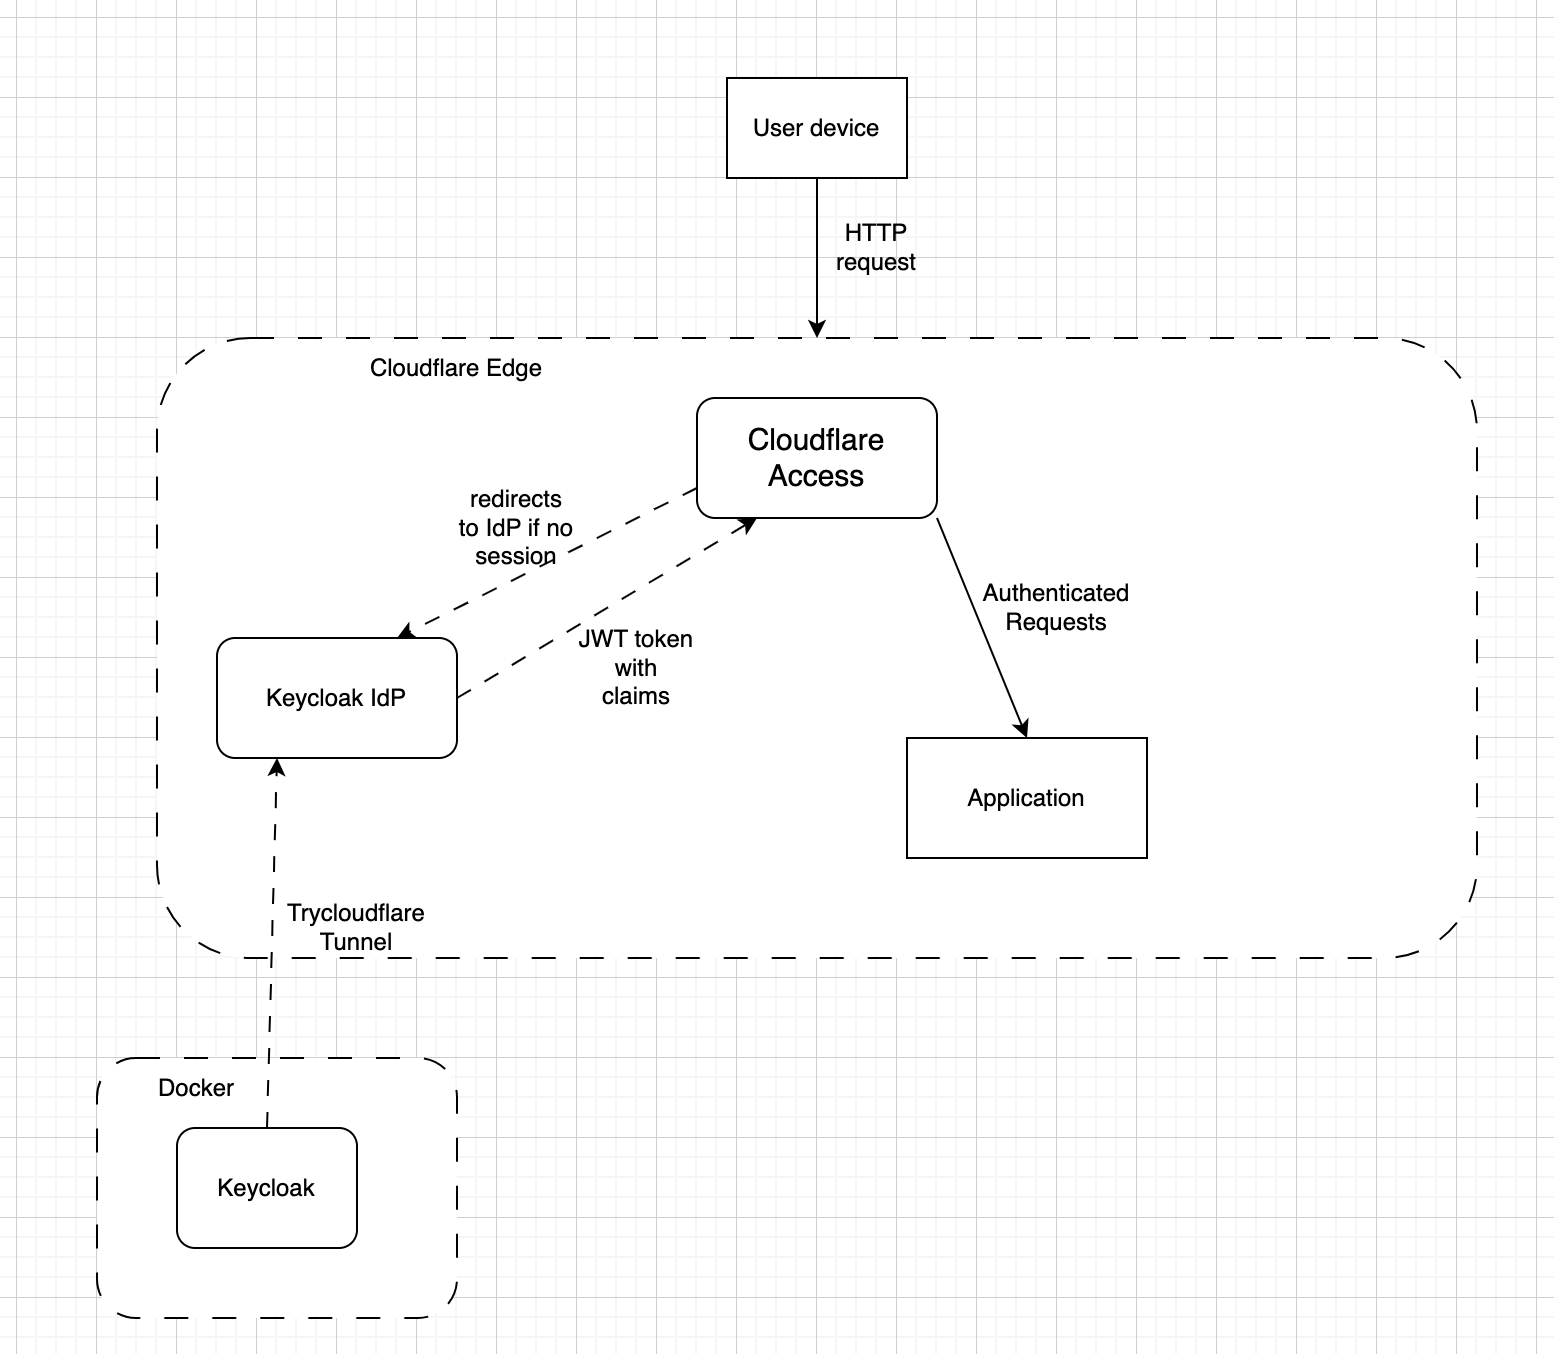
\includegraphics[width=0.5\textwidth]{contents/contents/image_11.png}
    \caption{Luồng thực thi của hệ thống}
    \label{fig:example_image}
    
\end{figure}

\subsection{Thiết kế kỹ thuật và đặc trưng}
Vì ứng dụng chạy ngay trên Worker, việc phân quyền không cần qua một "đường ống" nào mà được xử lý trực tiếp bằng code:

Đầu vào: Yêu cầu gồm các tiêu đề(headers) chứa các thông tin định danh đã được Cloudflare Access xác thực và lấy được thông qua claim dữ liệu từ keycloak.

Logic: Sử dụng mã JavaScript/TypeScript để kiểm tra quyền hạn (ví dụ: if (groups.includes('admin')) { ... }).

Zero Infrastructure: Không cần quản lý server, không cần lo về Tunnel hay mở port.

Tính sẵn sàng cao: Ứng dụng chạy trên hạ tầng toàn cầu của Cloudflare, tự động mở rộng theo lượng truy cập.

Bảo mật: Code chỉ chạy sau khi đã qua lớp lọc của Cloudflare Access. Nếu không có token hợp lệ, ngay cả yêu cầu cũng không đến được worker.

\subsection{Đánh giá giải pháp thiết kế}

Việc lựa chọn thiết kế này mang lại các giá trị thực tiễn vượt trội so với mô hình truyền thống:

\begin{table}[H]
\centering
\caption{Đánh giá giải pháp thiết kế dựa trên nhu cầu thực tế}
\label{tab:design_evaluation}
\renewcommand{\arraystretch}{1.5}
% Đảm bảo đã khai báo \usepackage[table]{xcolor} ở đầu file
\begin{tabular}{|p{3.5cm}|p{5cm}|p{5.5cm}|}
\hline
\textbf{Vấn đề đặt ra} & \textbf{Giải pháp thiết kế} & \textbf{Kết quả đạt được} \\ \hline
Nguy cơ lộ IP máy chủ & Chạy trực tiếp trên Workers & Không có máy chủ vật lý, không có IP để tấn công. \\ \hline
Độ trễ khi xác thực & Sử dụng QUIC Domain cho IdP & Tối ưu hóa tốc độ điều hướng và bắt tay TLS. \\ \hline
Phân quyền phức tạp & Phân quyền dựa trên tiêu đề claims từ danh tính người dùng & Phân quyền trực tiếp trong code dựa trên Claim từ Keycloak. \\ \hline
Chi phí hạ tầng & Serverless Model & Không tốn chi phí vận hành, bảo trì máy chủ 24/7. \\ \hline
\end{tabular}
\end{table}
\section{Hiện thực và đánh giá}
\subsection{Khởi tạo Keycloak realm}
\begin{itemize}
    \item \textbf{Mục tiêu}: Cung cấp một luồng xác thực tập trung, trong đó Keycloak đóng vai trò Identity Provider (IdP) còn Cloudflare Access đóng vai trò lớp kiểm soát truy cập ở biên mạng.
    \item \textbf{Phạm vi}: Thử nghiệm trên môi trường sử dụng \texttt{trycloudflare} để công bố tạm thời dịch vụ Keycloak ra Internet phục vụ quá trình tích hợp và đánh giá.
    \item \textbf{Kết quả mong đợi}: Người dùng phải đăng nhập qua Keycloak trước khi được Cloudflare cấp quyền truy cập ứng dụng được bảo vệ.
\end{itemize}

\subsection{Khởi chạy \texttt{trycloudflare} để công bố Keycloak}
Giai đoạn đầu tiên là đưa dịch vụ Keycloak nội bộ ra một địa chỉ công khai tạm thời để Cloudflare Zero Trust có thể truy cập các endpoint OIDC.
\begin{itemize}
    \item Khởi chạy Keycloak trên máy chủ nội bộ với Realm phục vụ thử nghiệm (zta-lab).
    \item Sử dụng \texttt{cloudflared tunnel --url http://localhost:<port>} để tạo một free tunnel công khai qua miền \texttt{trycloudflare.com}.
    \item Ghi nhận URL được cấp phát để sử dụng làm \textit{Issuer}, \textit{Authorization Endpoint}, \textit{Token Endpoint} và \textit{JWKS Endpoint} trong quá trình tích hợp.
    \item Kiểm tra khả năng truy cập từ bên ngoài nhằm bảo đảm các endpoint OIDC của Keycloak hoạt động ổn định.
\end{itemize}

\subsection{Cấu hình Keycloak cho luồng OIDC}
Sau khi công bố dịch vụ thành công, tiến hành cấu hình Realm và Client trong Keycloak để cho phép Cloudflare sử dụng làm bên tin cậy xác thực.
\begin{itemize}
    \item Tạo Realm riêng cho hệ thống nhằm tách biệt người dùng, vai trò và chính sách với các môi trường khác.
    \item Tạo Client theo chuẩn OpenID Connect, thiết lập \textit{redirect URI} trỏ về đường dẫn callback do Cloudflare Access cung cấp.
    \item Khai báo \textit{client ID}, \textit{client secret}, phạm vi truy cập và ánh xạ các thuộc tính người dùng cần đưa vào token thông qua các client scope và mapper.
    \item Tạo người dùng thử nghiệm, nhóm hoặc vai trò để phục vụ cho bước xây dựng chính sách truy cập phía Cloudflare.
\end{itemize}
\begin{figure}[H]
    \centering
    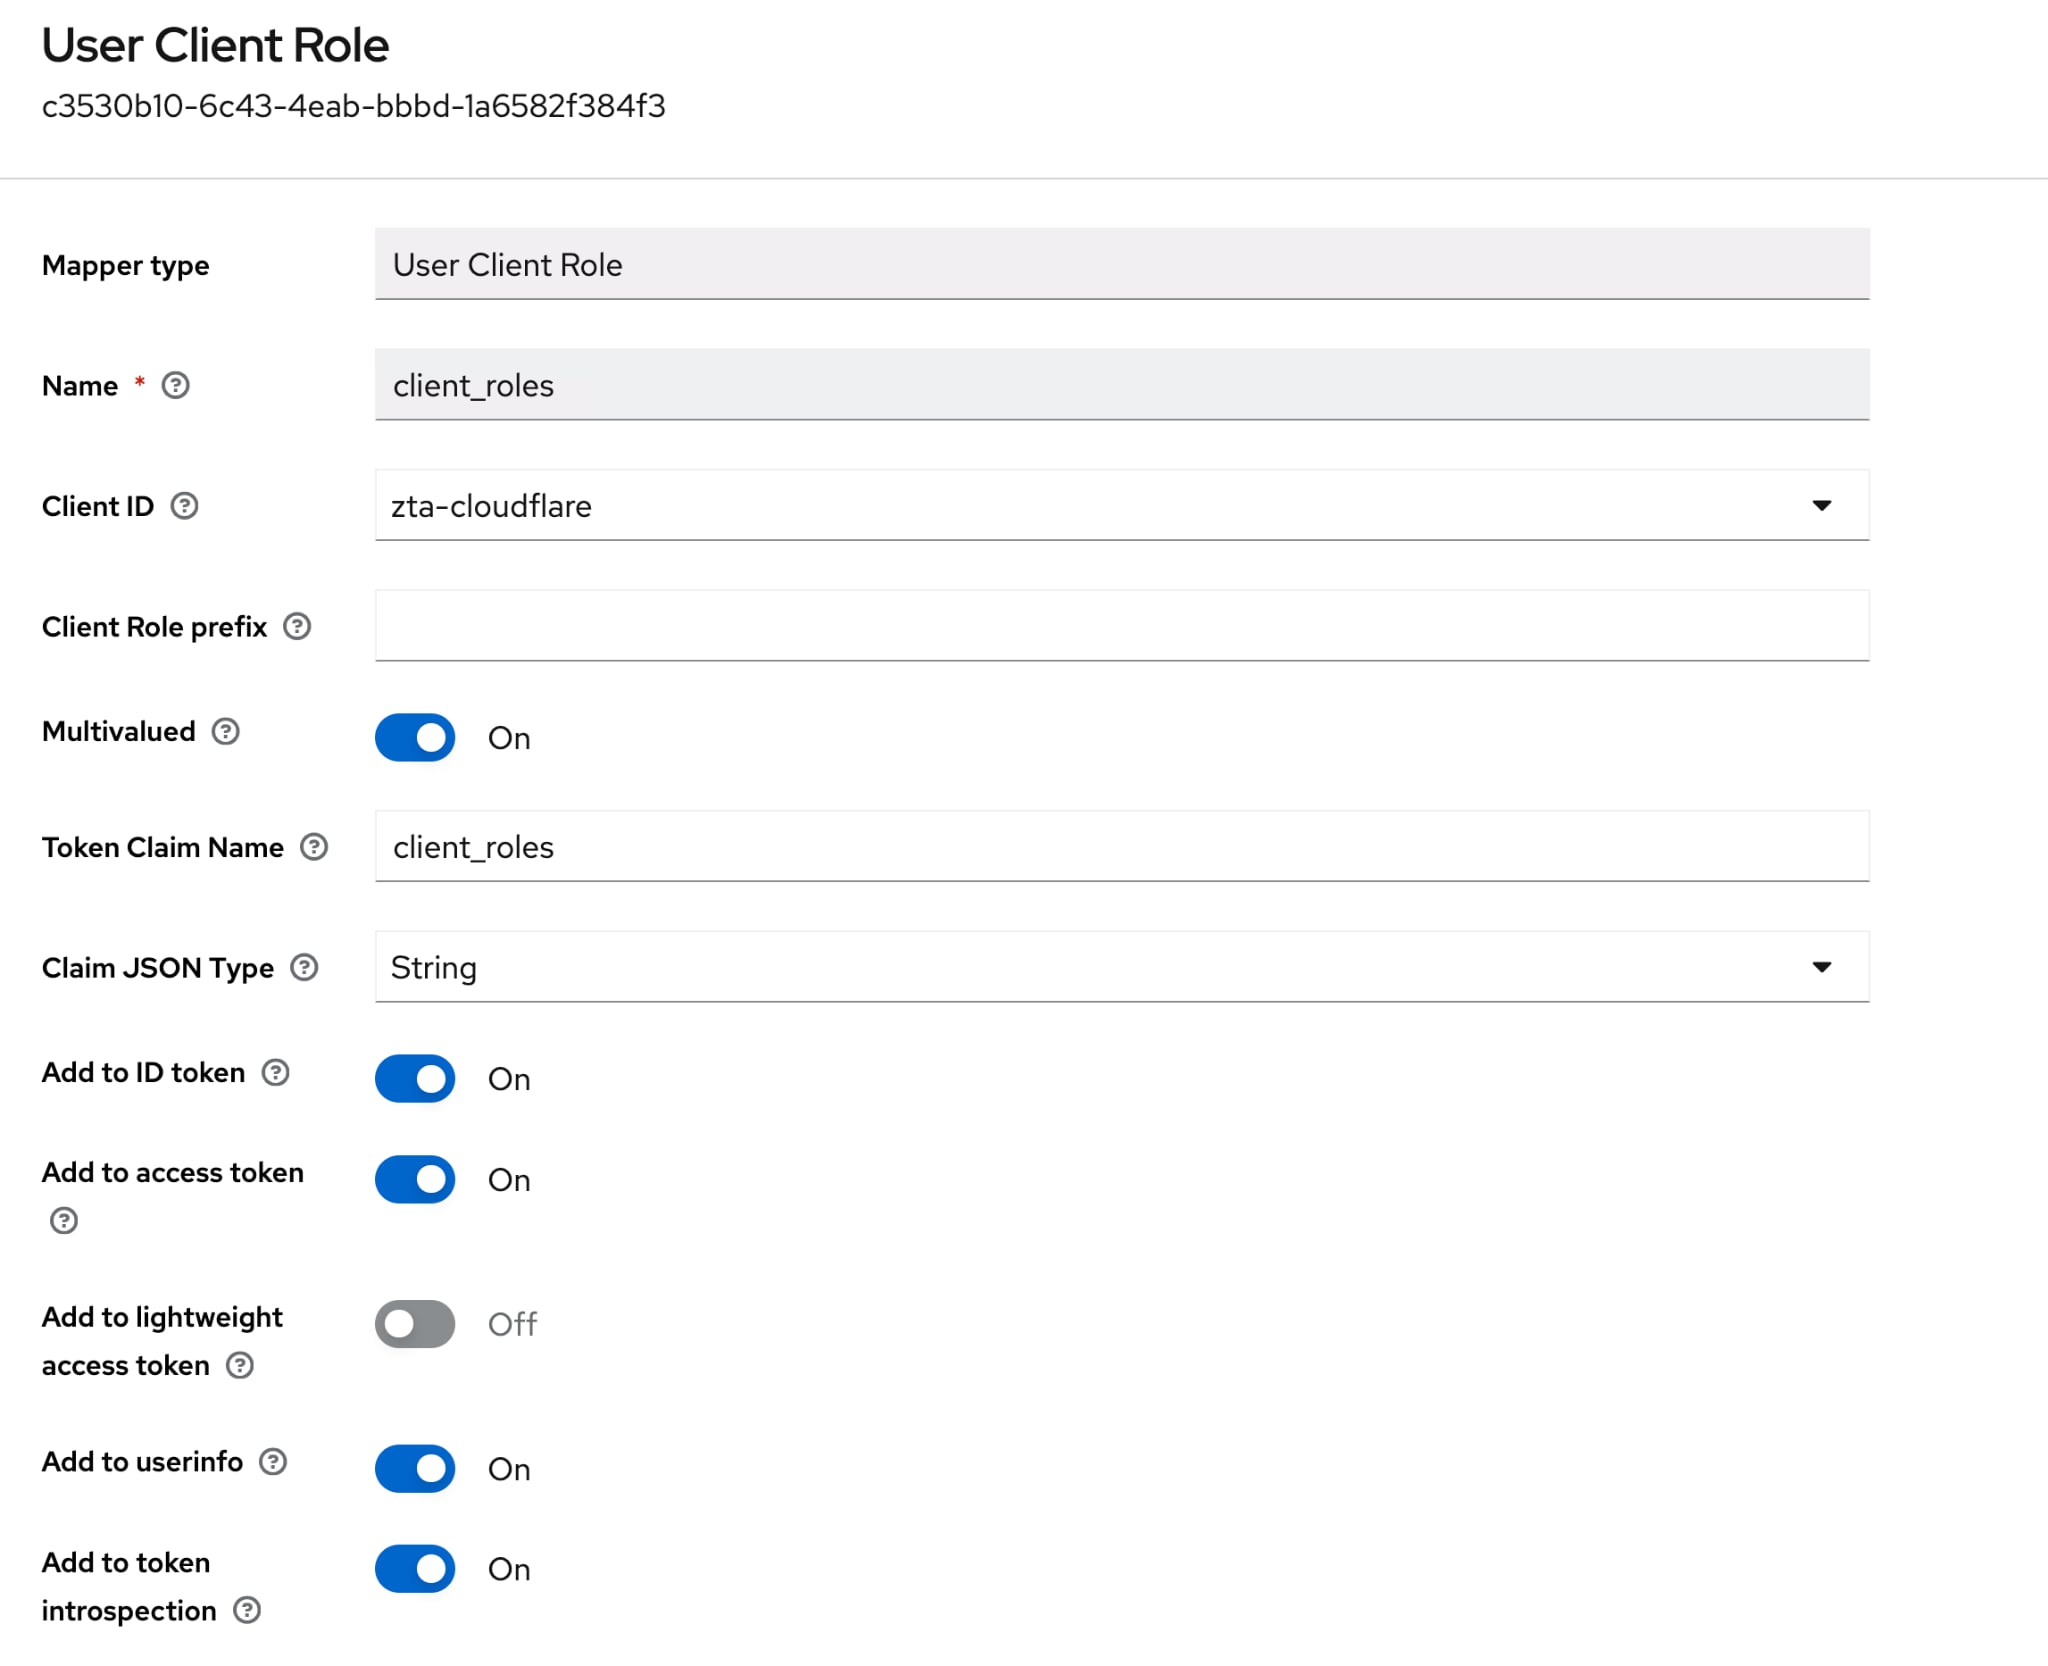
\includegraphics[width=0.5\textwidth]{contents/contents/image_7.png}    
    \caption{Mapper cho Client Role}
    \label{fig:example_image}
    
\end{figure}
 
\begin{figure}[H]
    \centering
    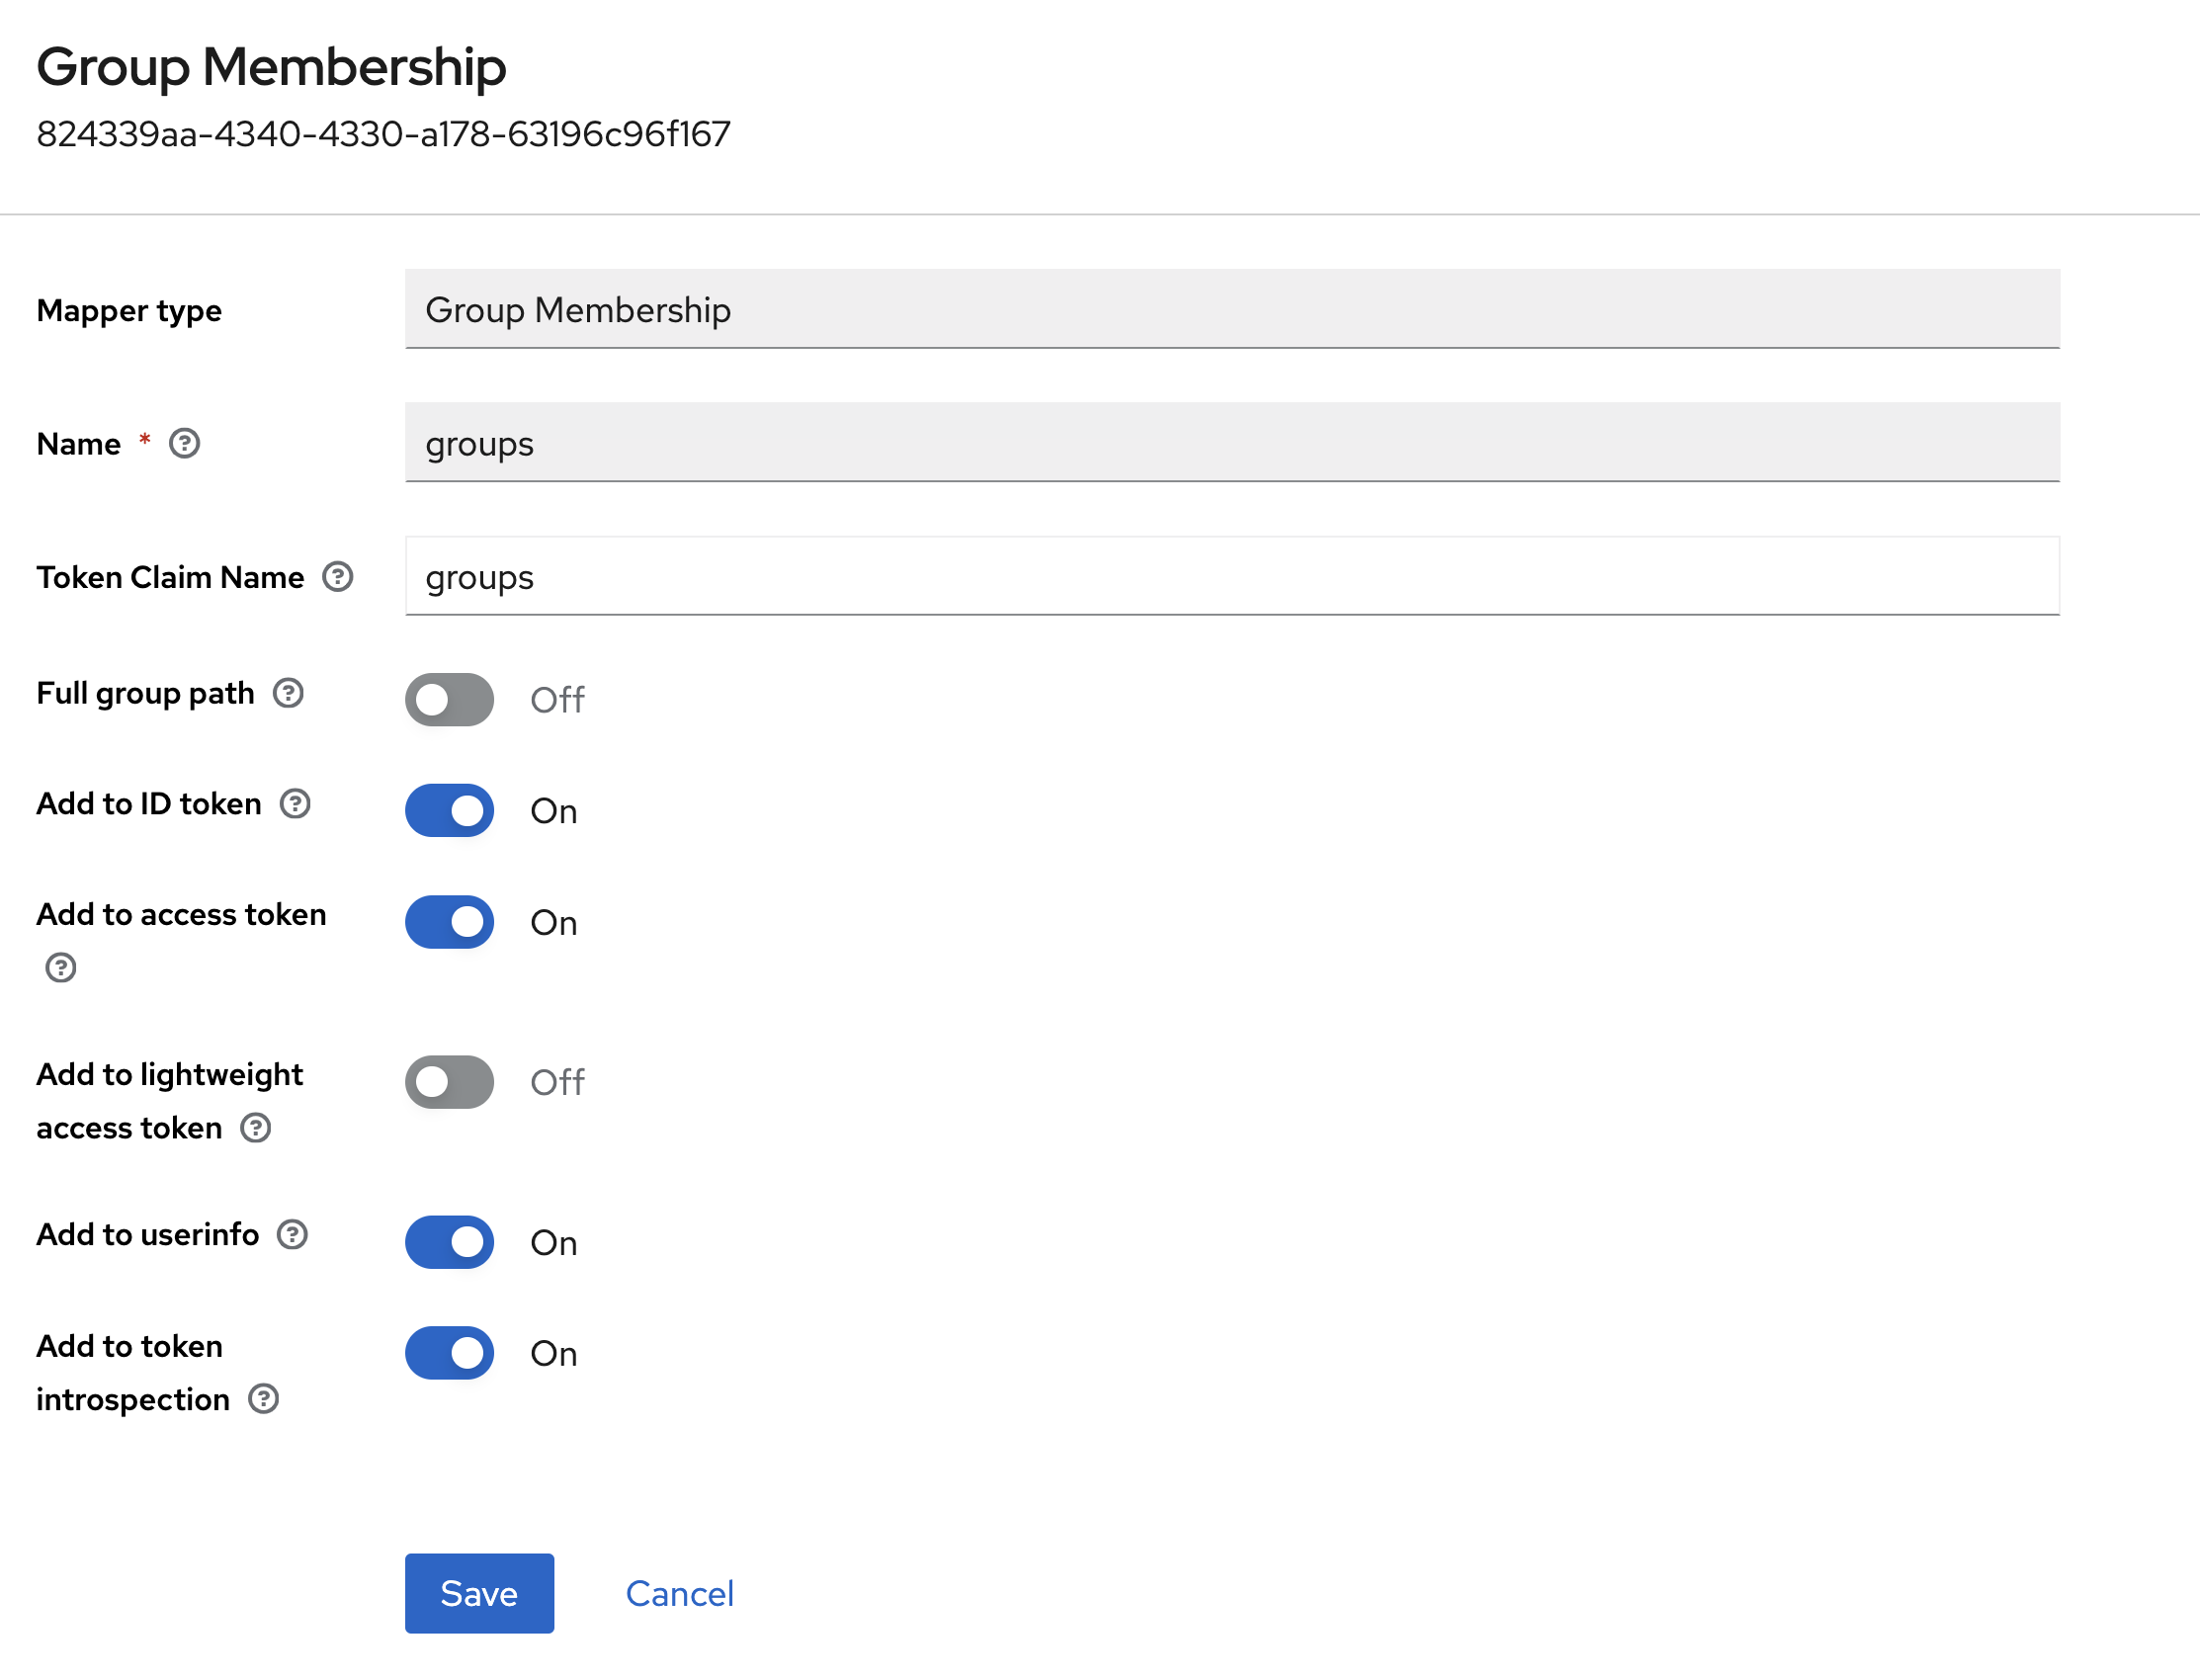
\includegraphics[width=0.5\textwidth]{contents/contents/image_9.png}
    \caption{Mapper cho Group Membership}
    \label{fig:example_image}
    
\end{figure}

Các nội dung dùng để xác minh danh tính được claims thông qua các mapper được tạo bên trên lấy tên, token claim name và loại dữ liệu phù hợp tương ứng. Ví dụ tên groups, token claimname là group và mapper type là group membership 
\begin{figure}[H]
    \centering
    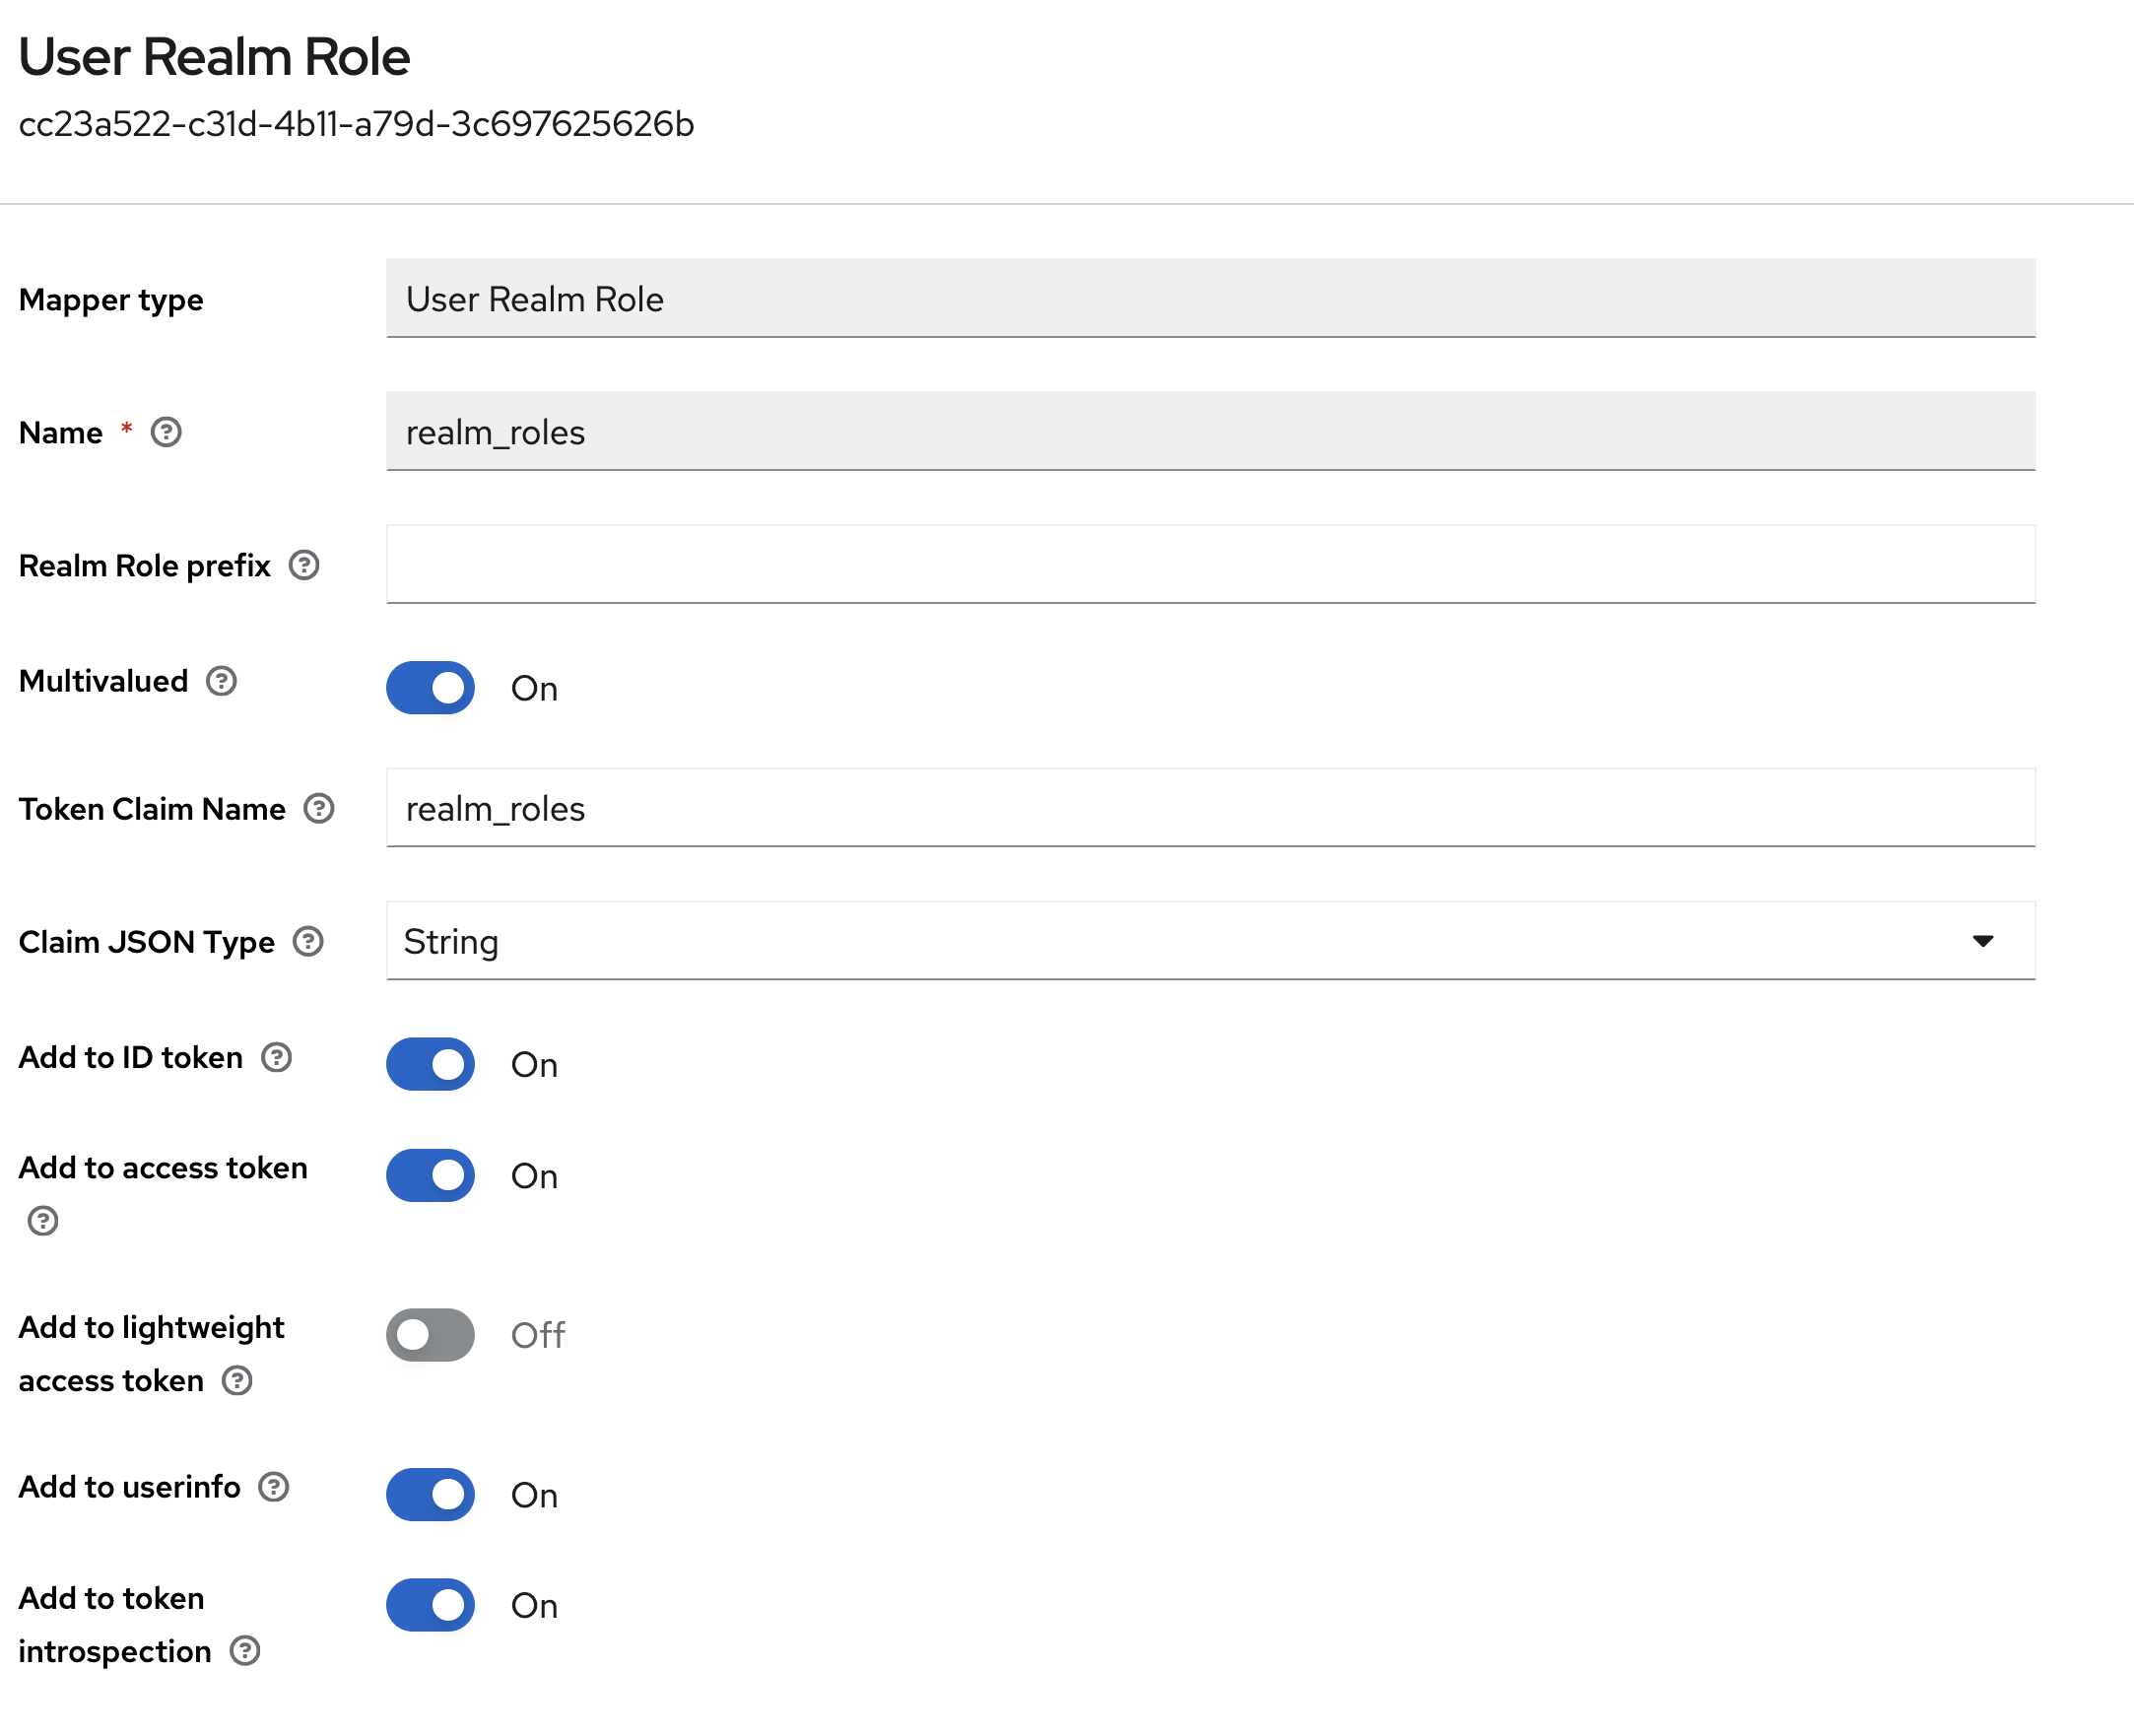
\includegraphics[width=0.5\textwidth]{contents/contents/image_10.png}
    \caption{Mapper cho User Realm Role}
    \label{fig:example_image}
    
\end{figure}

\begin{figure}[H]
    \centering
    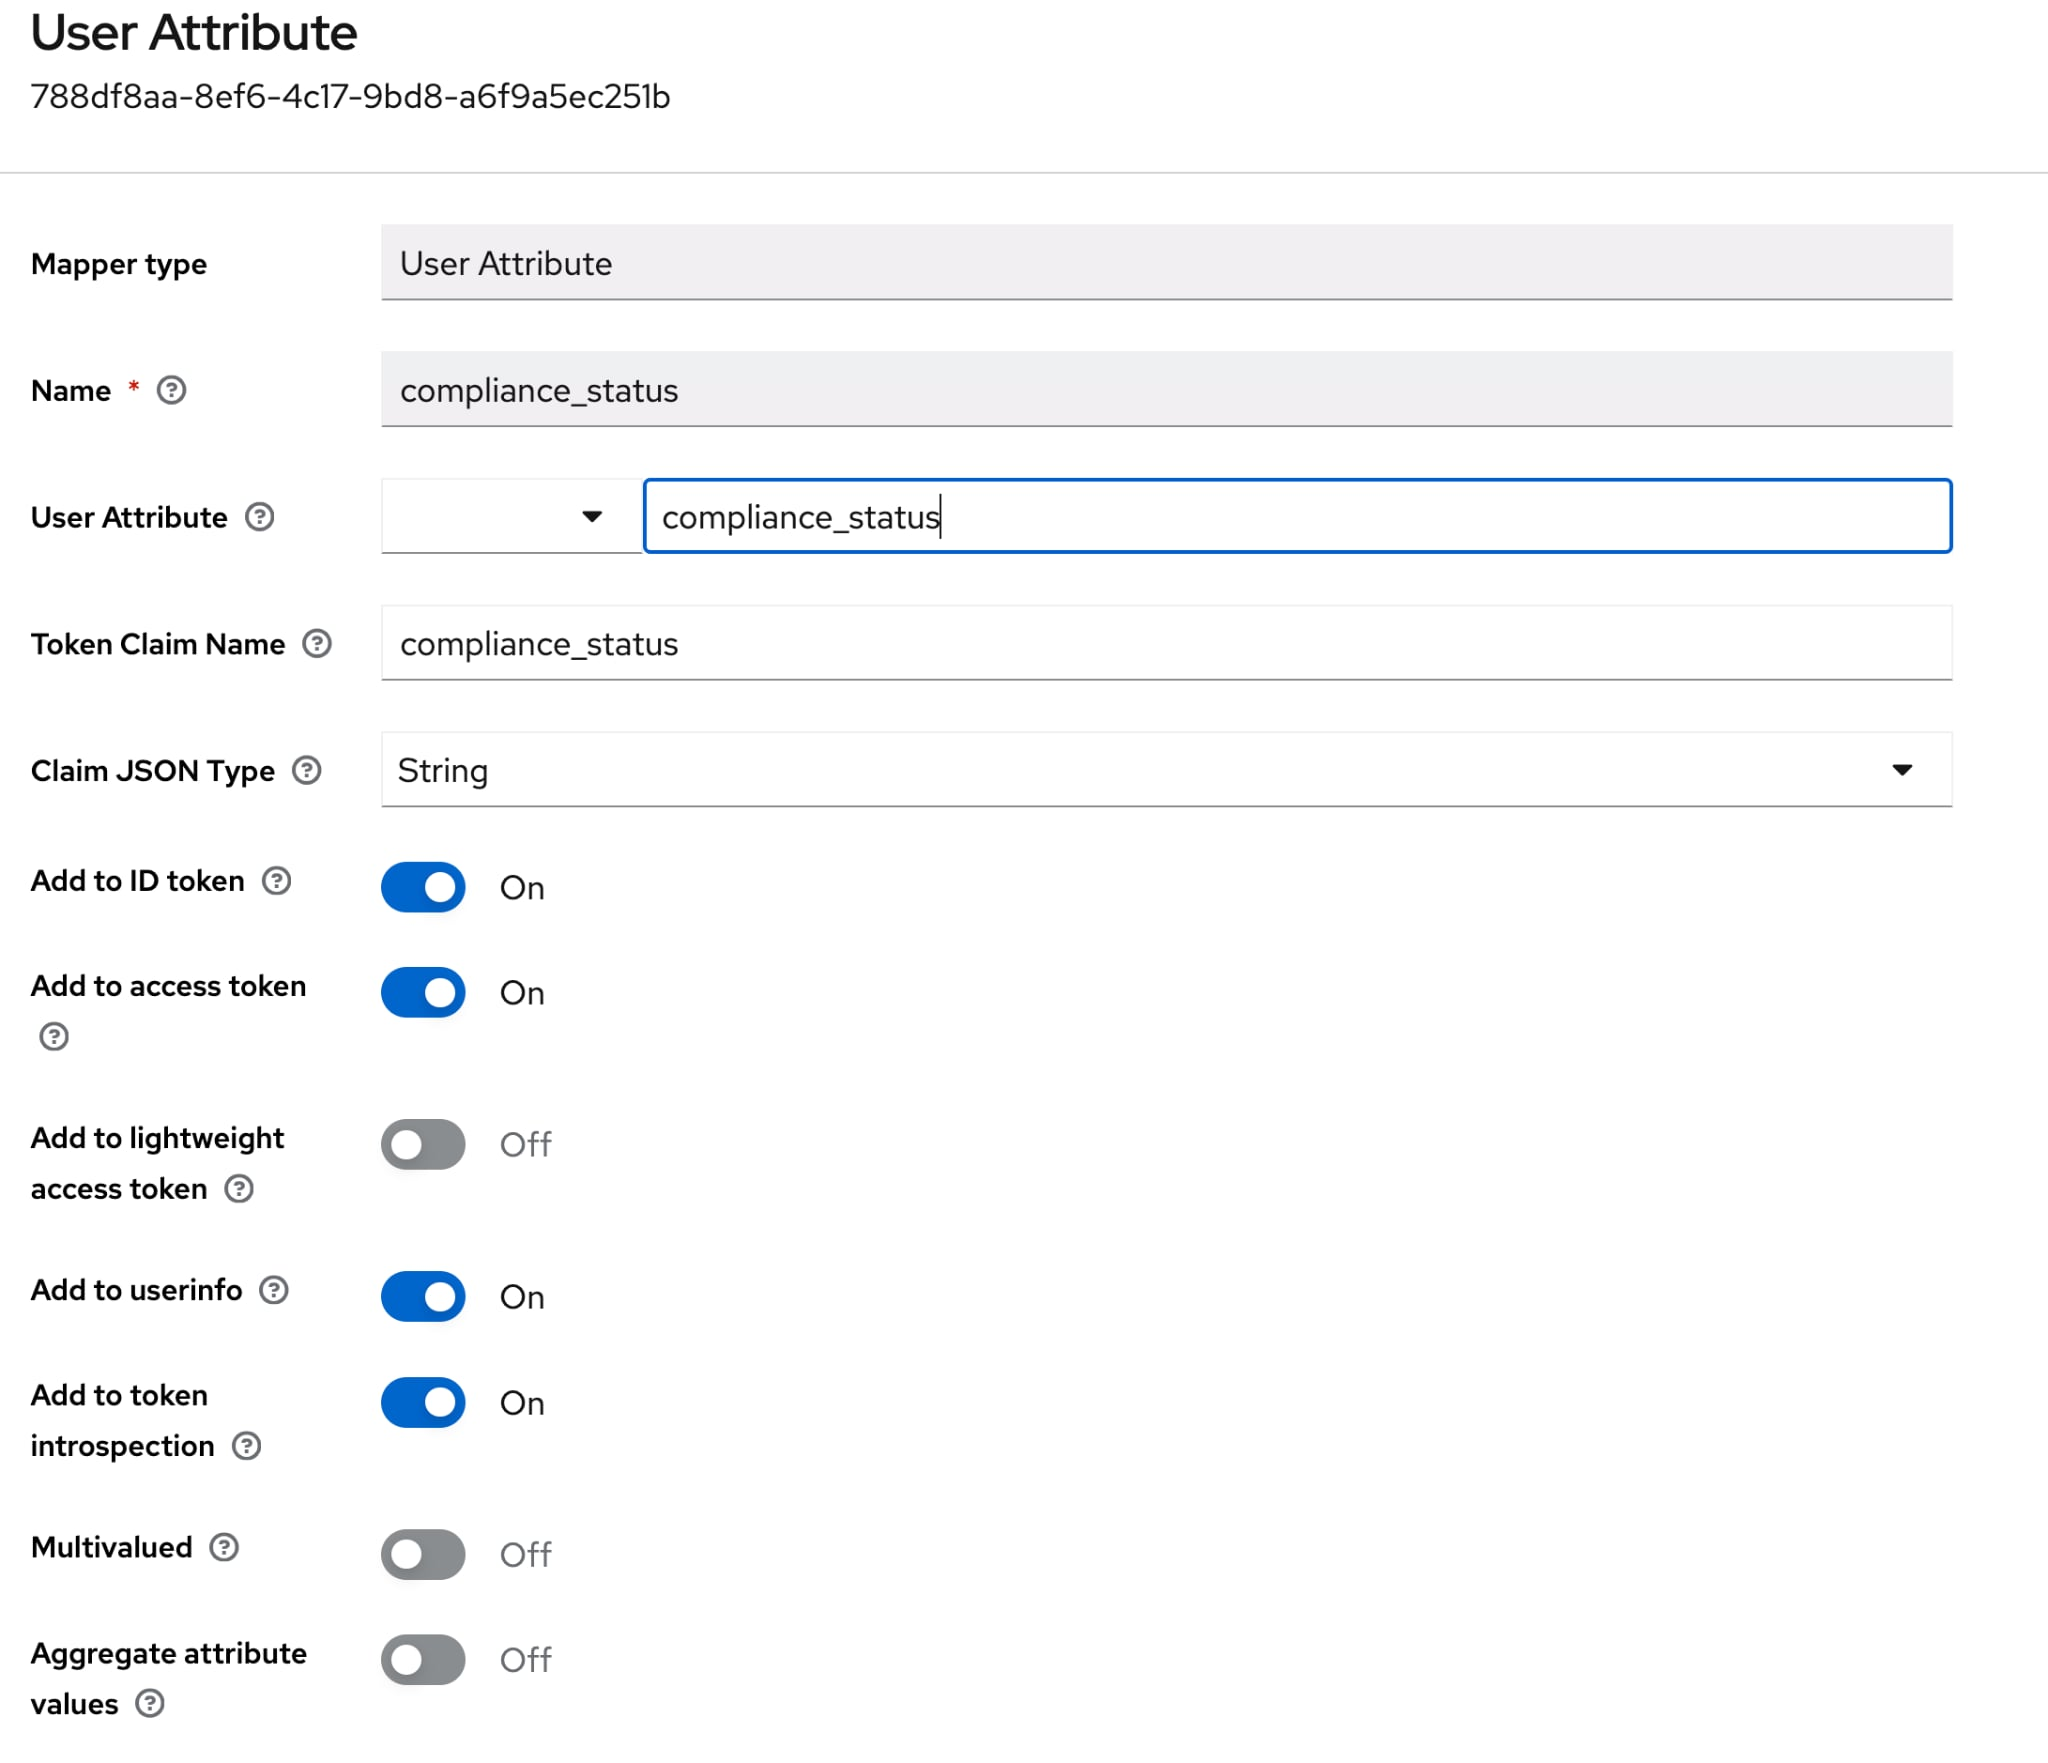
\includegraphics[width=0.5\textwidth]{contents/contents/image_8.png}
    \caption{Các Mapper cho User Attribute}
    \label{fig:example_image}
    
\end{figure}

\begin{figure}[H]
    \centering
    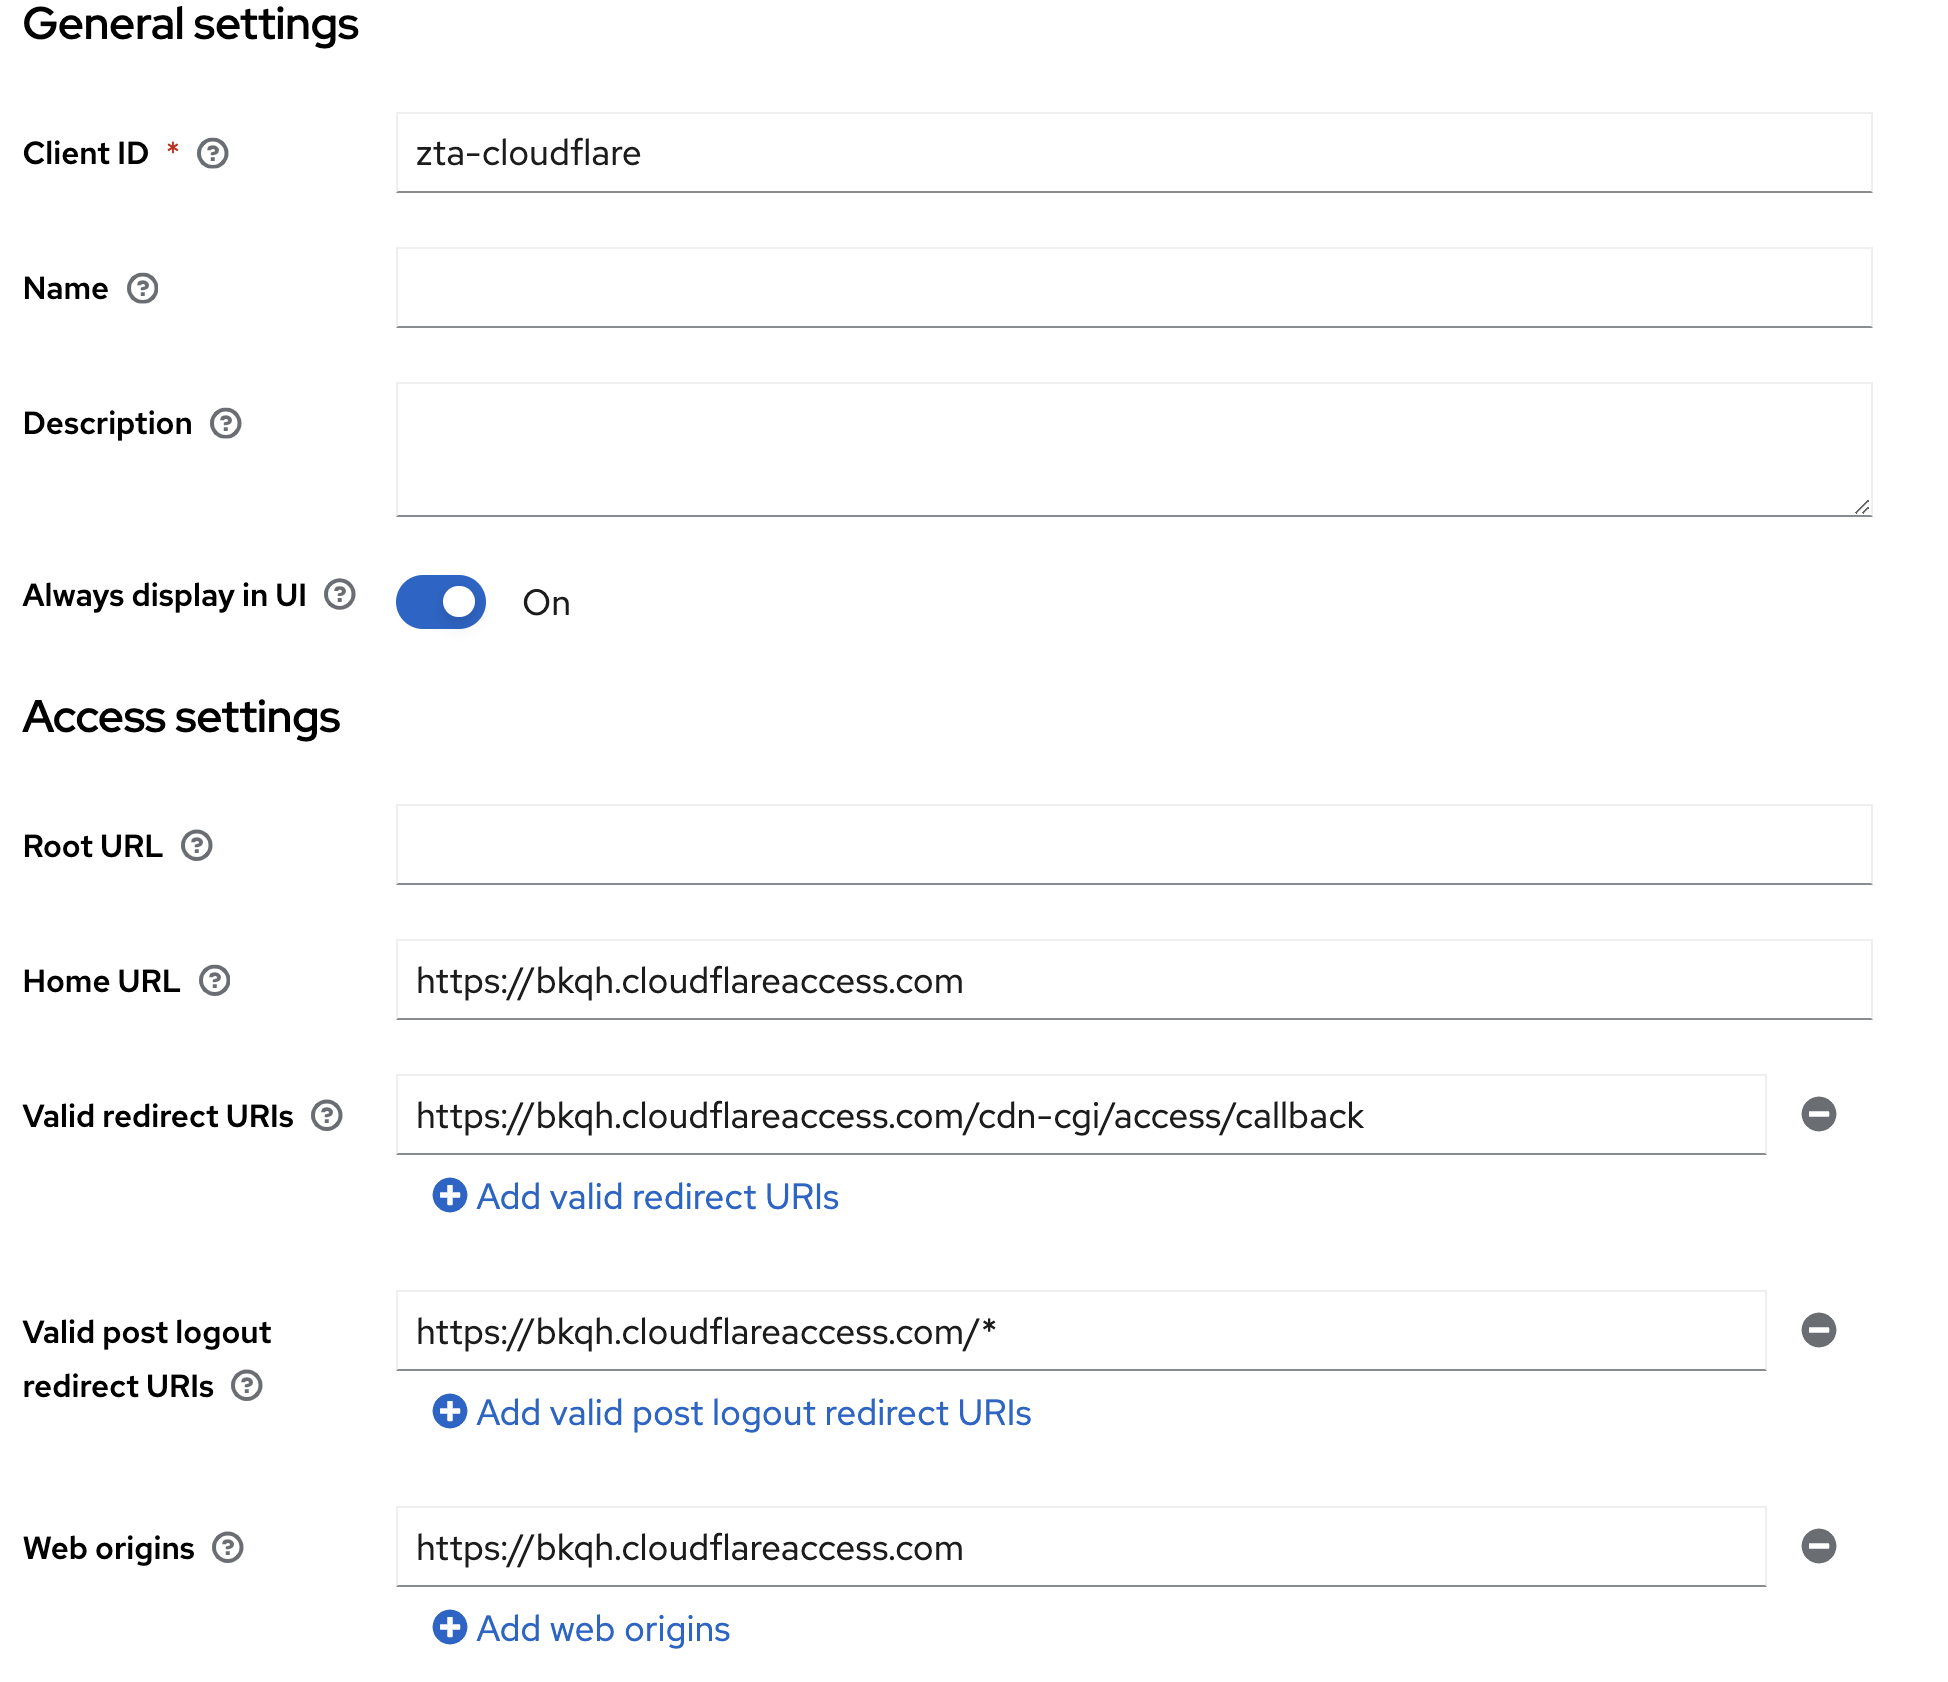
\includegraphics[width=0.8\textwidth]{contents/contents/image_2.png}
    \caption{Cấu hình cho Keycloak Client}
    \label{fig:example_image}
    
\end{figure}
\begin{figure}[H]
    \centering
    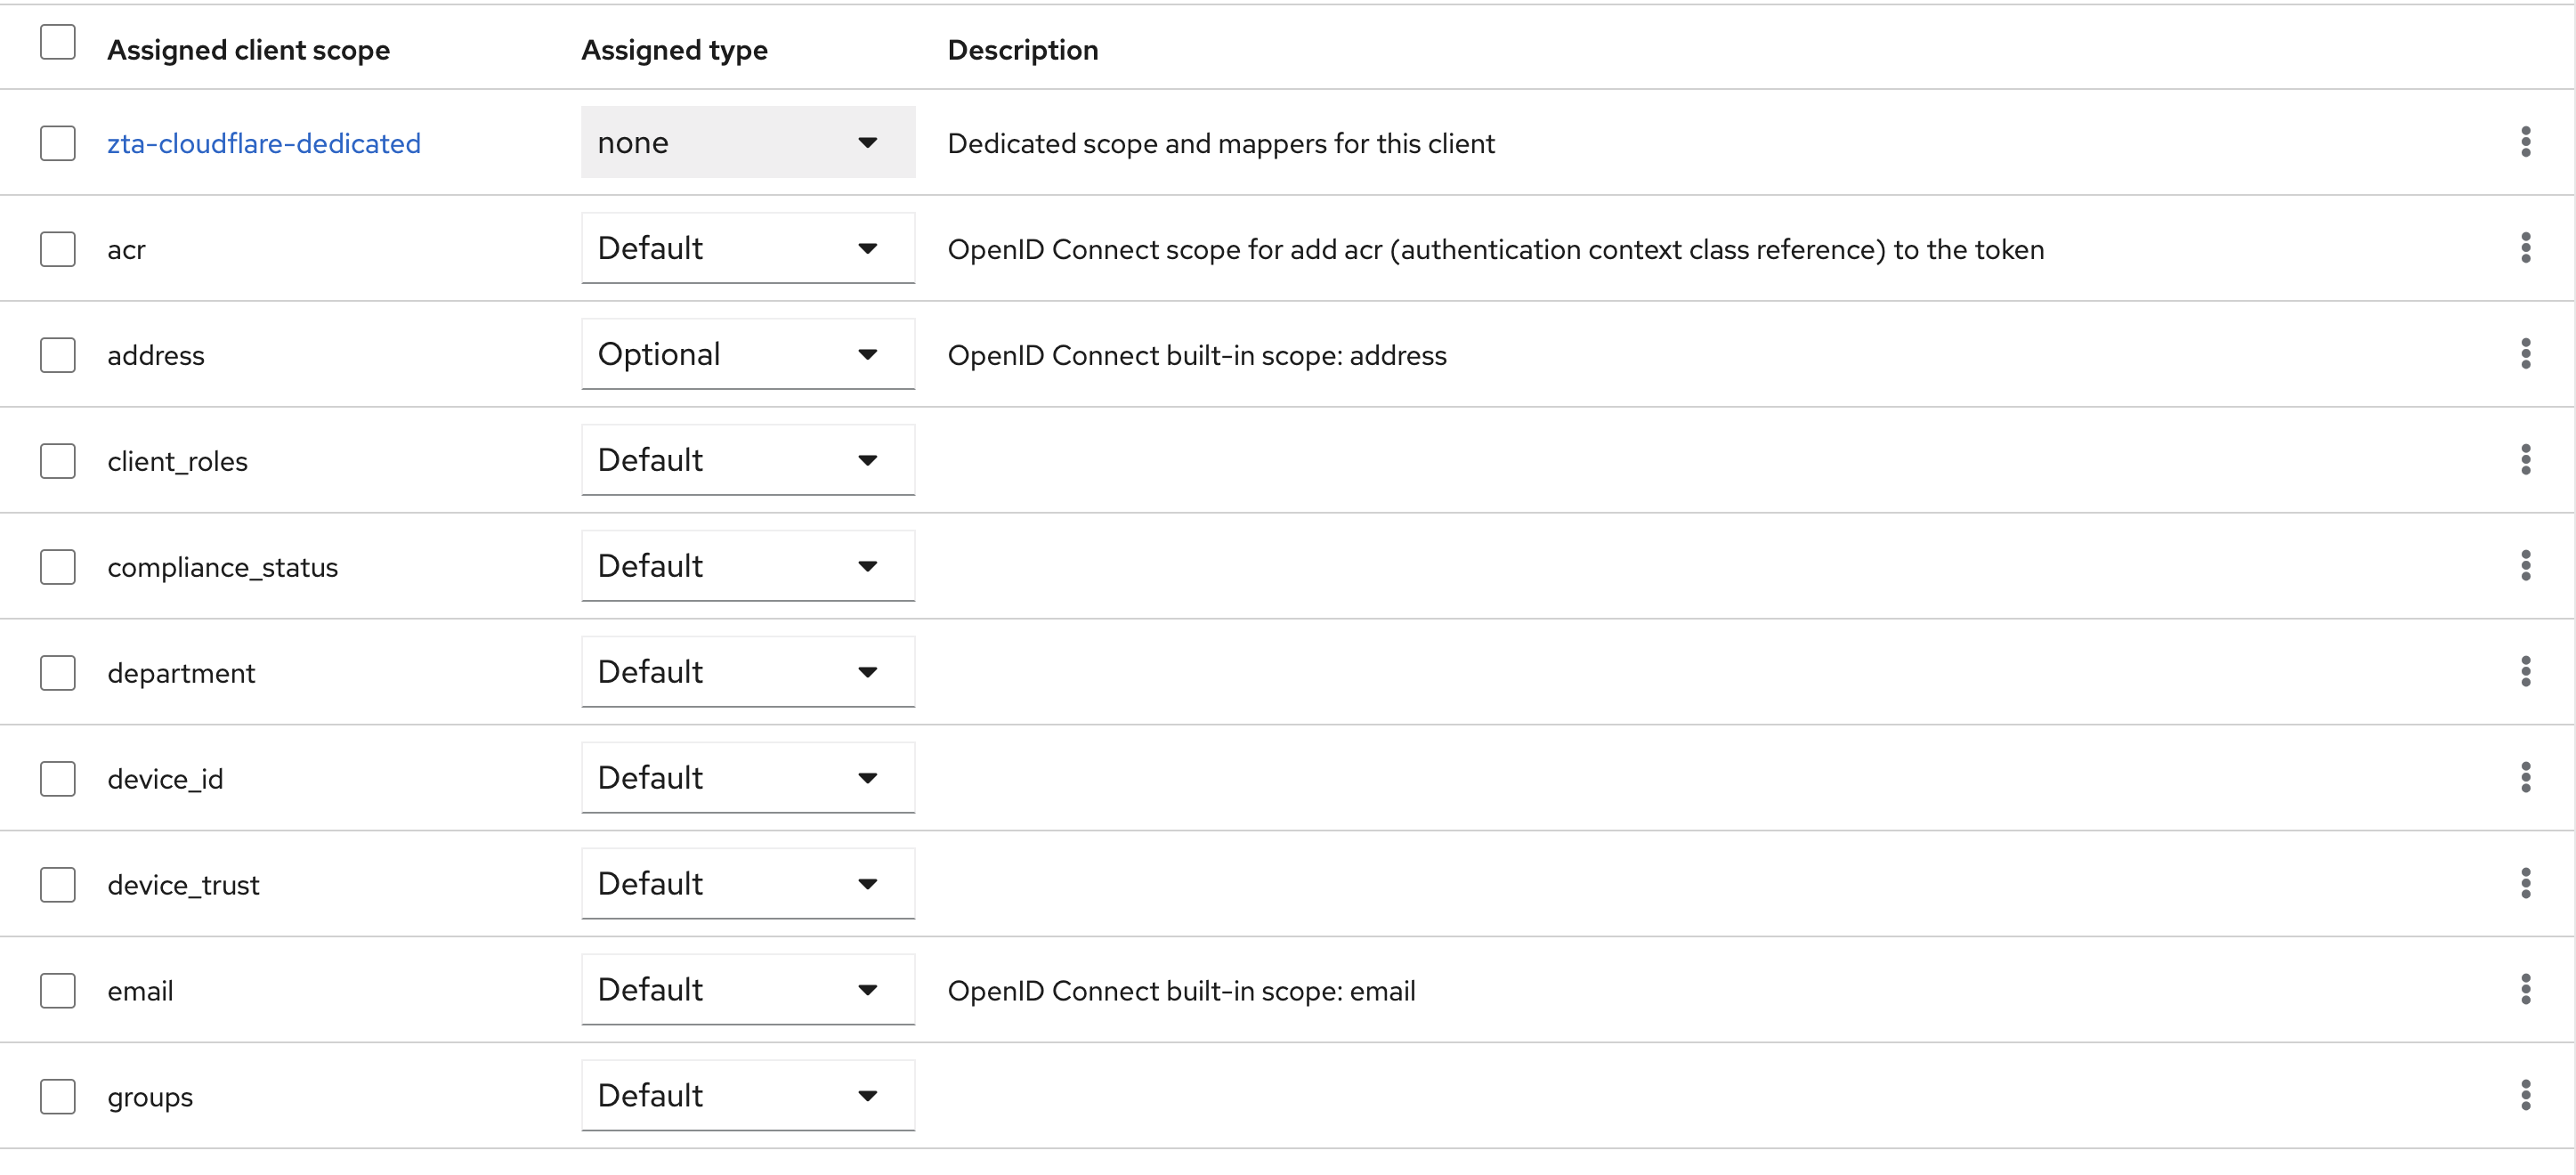
\includegraphics[width=0.5\textwidth]{contents/contents/image_3.png}    
    \caption{Cấu hình client scope}
    \label{fig:example_image}
    
\end{figure}

\begin{figure}[H]
    \centering
    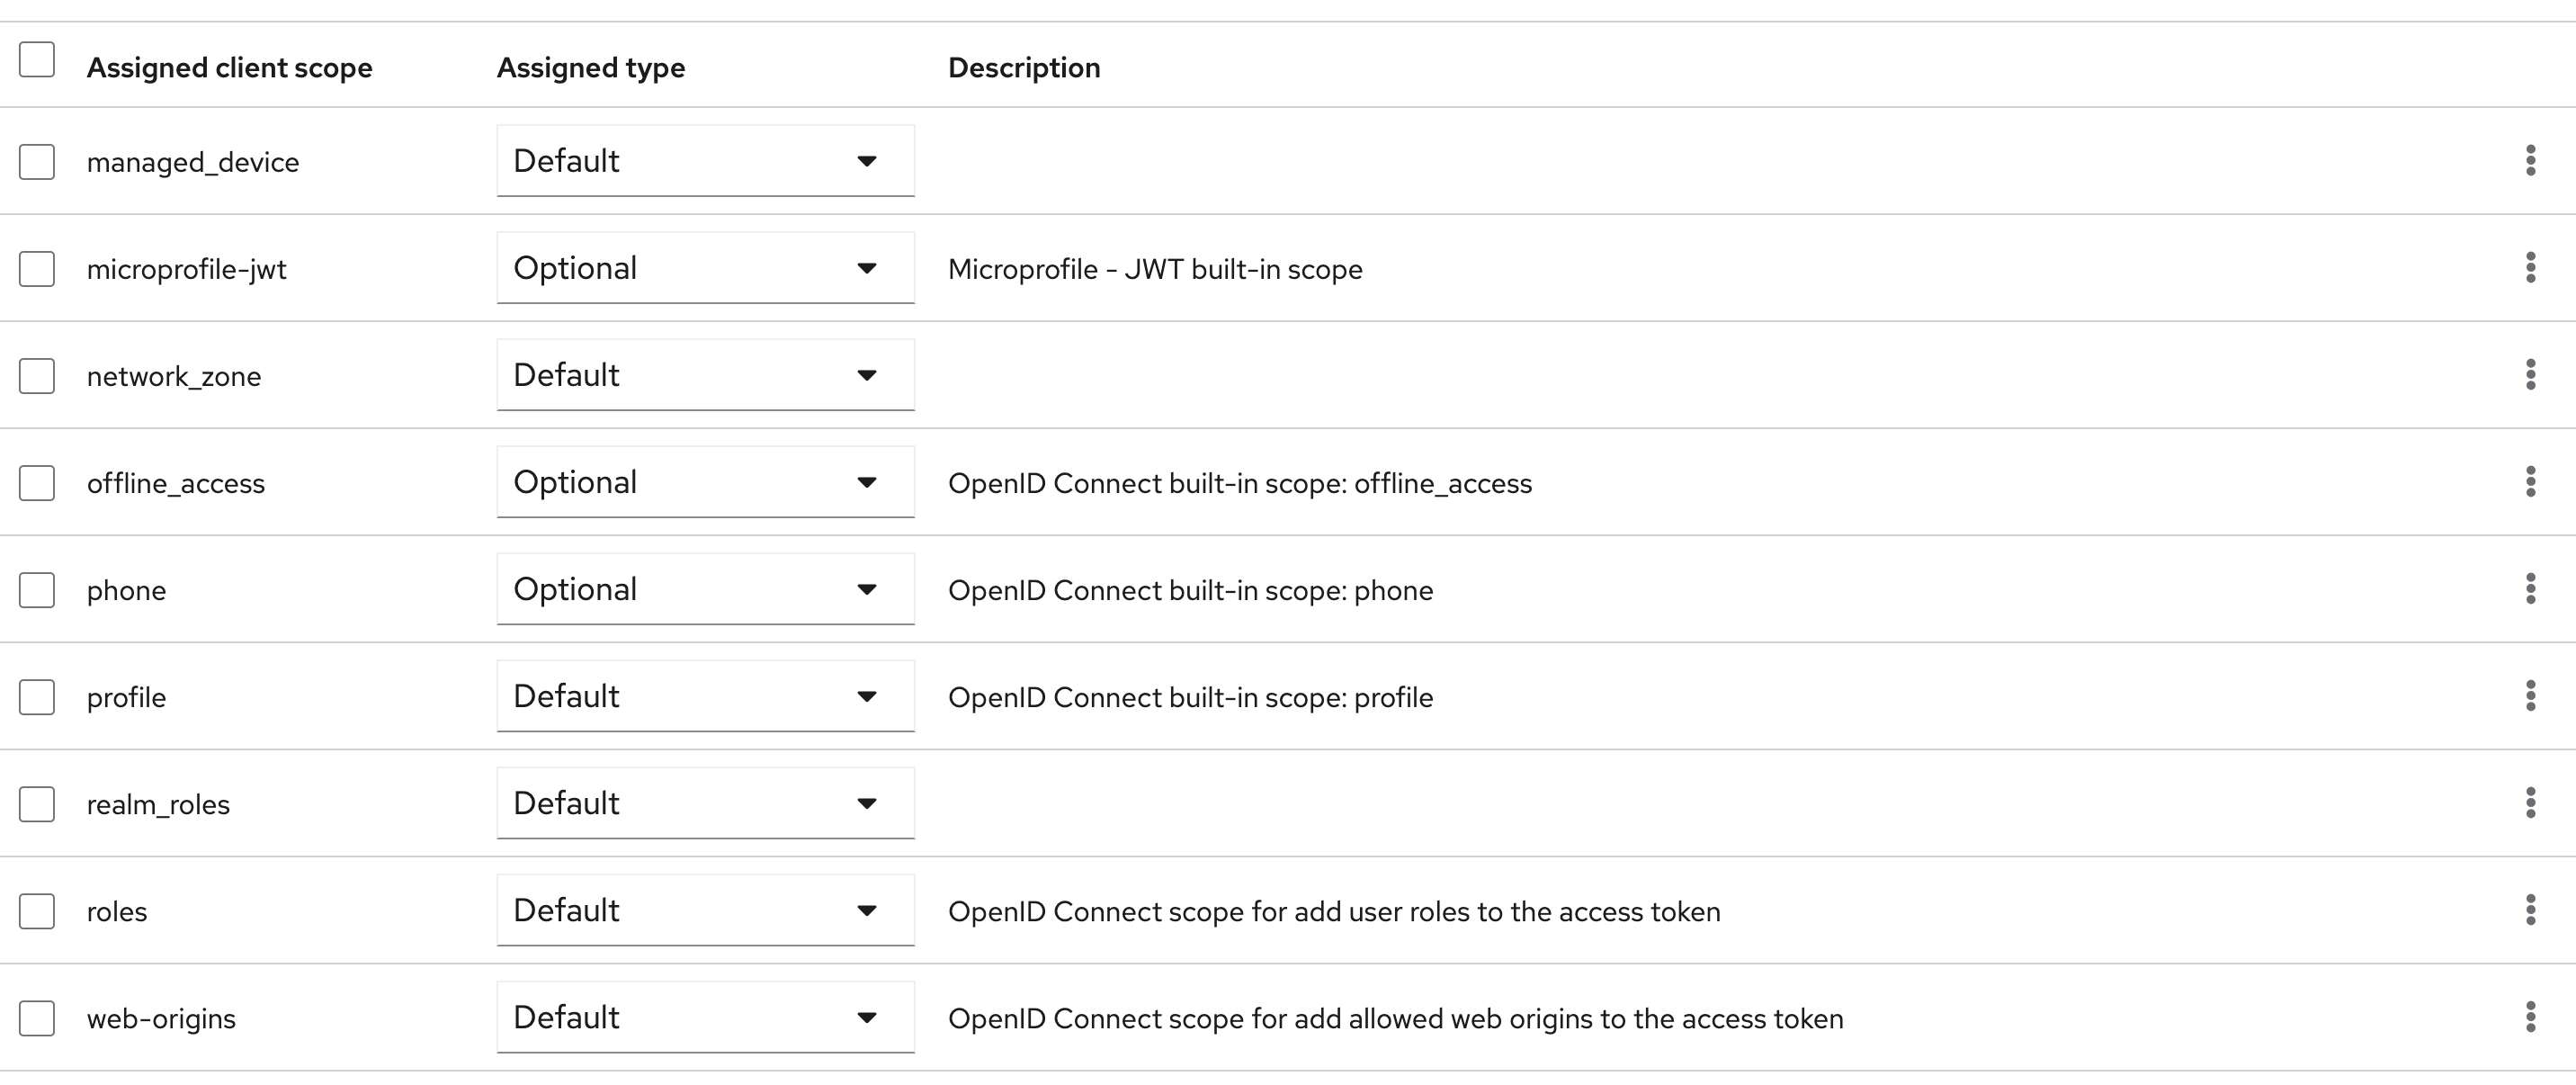
\includegraphics[width=0.5\textwidth]{contents/contents/image_4.png}    
    \caption{Cấu hình client scope}
    \label{fig:example_image}
    
\end{figure}

\begin{figure}[H]
    \centering
    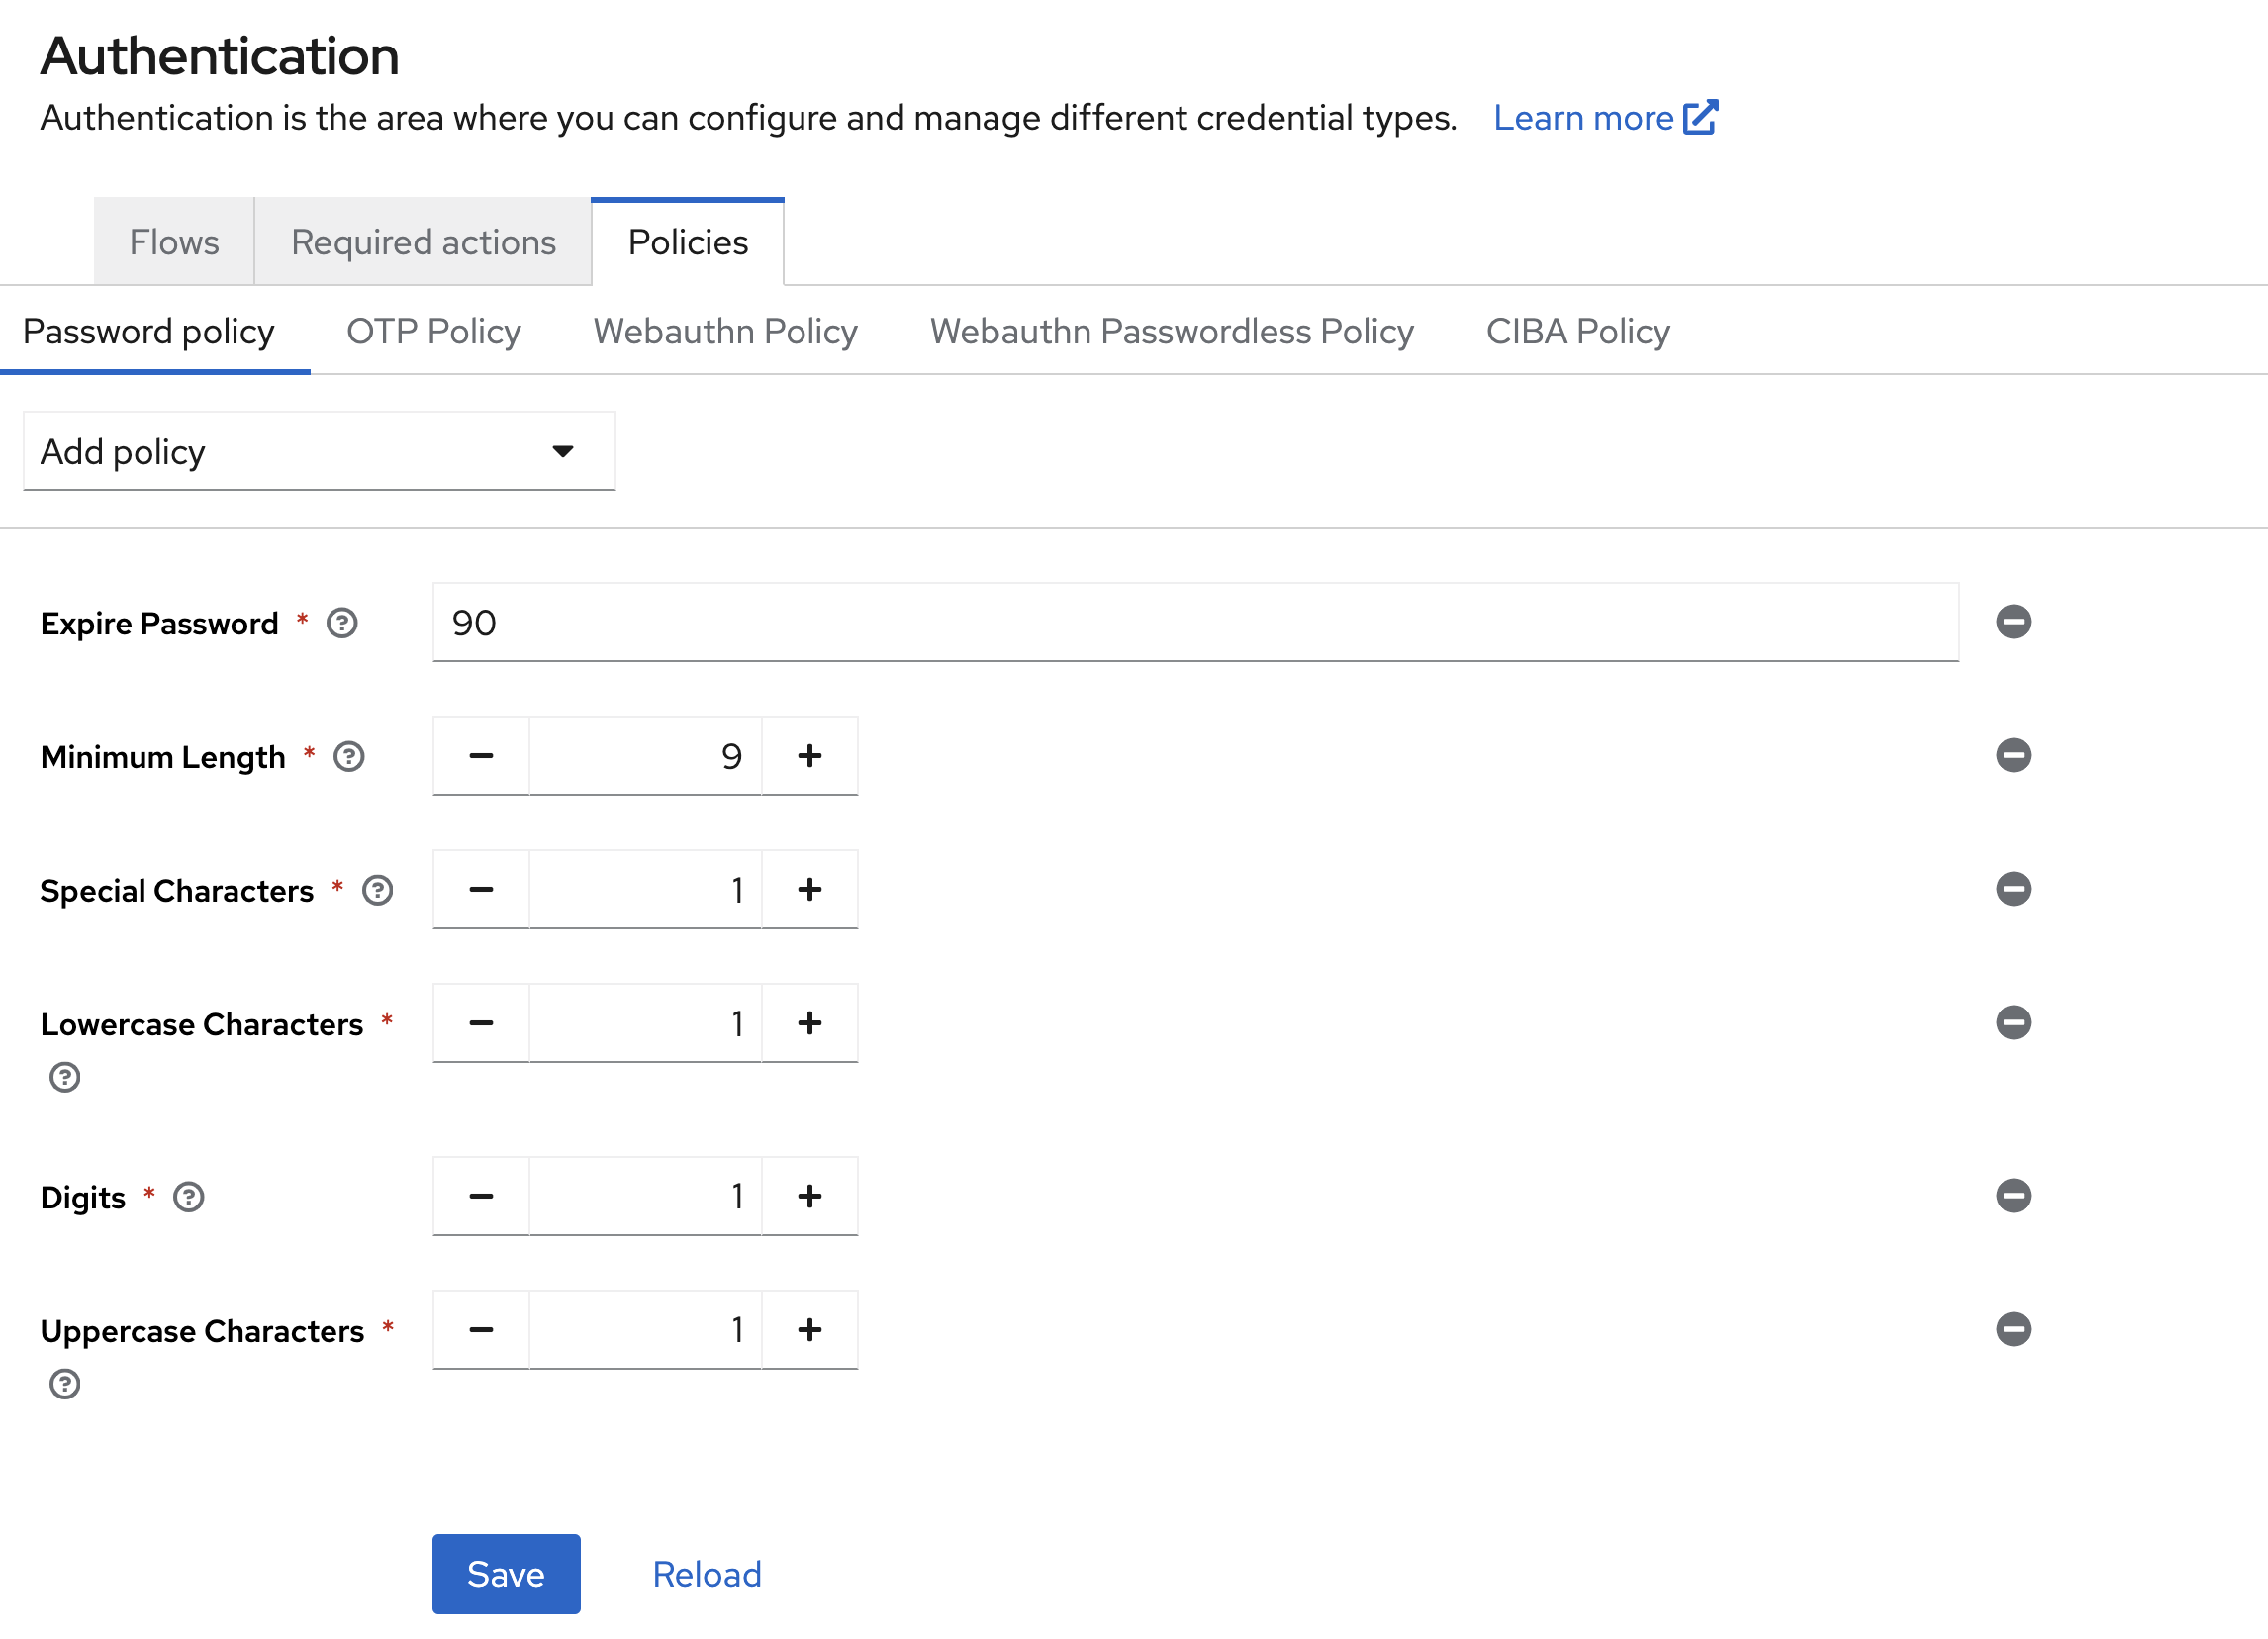
\includegraphics[width=0.5\textwidth]{contents/contents/image_16.png}
    \caption{Password policy cho người dùng}
    \label{fig:example_image}
    
\end{figure}

\subsection{Tích hợp Keycloak vào Cloudflare Zero Trust}
Ở bước này, Keycloak được khai báo như một nhà cung cấp danh tính OIDC cho hệ thống Cloudflare Zero Trust.
\begin{itemize}
    \item Truy cập mục quản lý Identity Providers trong Cloudflare Zero Trust và chọn thêm nhà cung cấp OIDC tùy chỉnh.
    \item Điền các tham số tích hợp gồm \textit{client ID}, \textit{client secret}, \textit{issuer URL} và các endpoint tương ứng lấy từ Keycloak qua tunnel công khai.
    \item Kiểm tra quá trình đồng bộ thông tin định danh để bảo đảm Cloudflare có thể chuyển hướng người dùng tới Keycloak và nhận lại token hợp lệ.
    \item Xác nhận các trường nhận dạng như email, username hoặc nhóm người dùng có thể được dùng làm điều kiện trong Access Policy.
\end{itemize}
\begin{figure}[H]
    \centering
    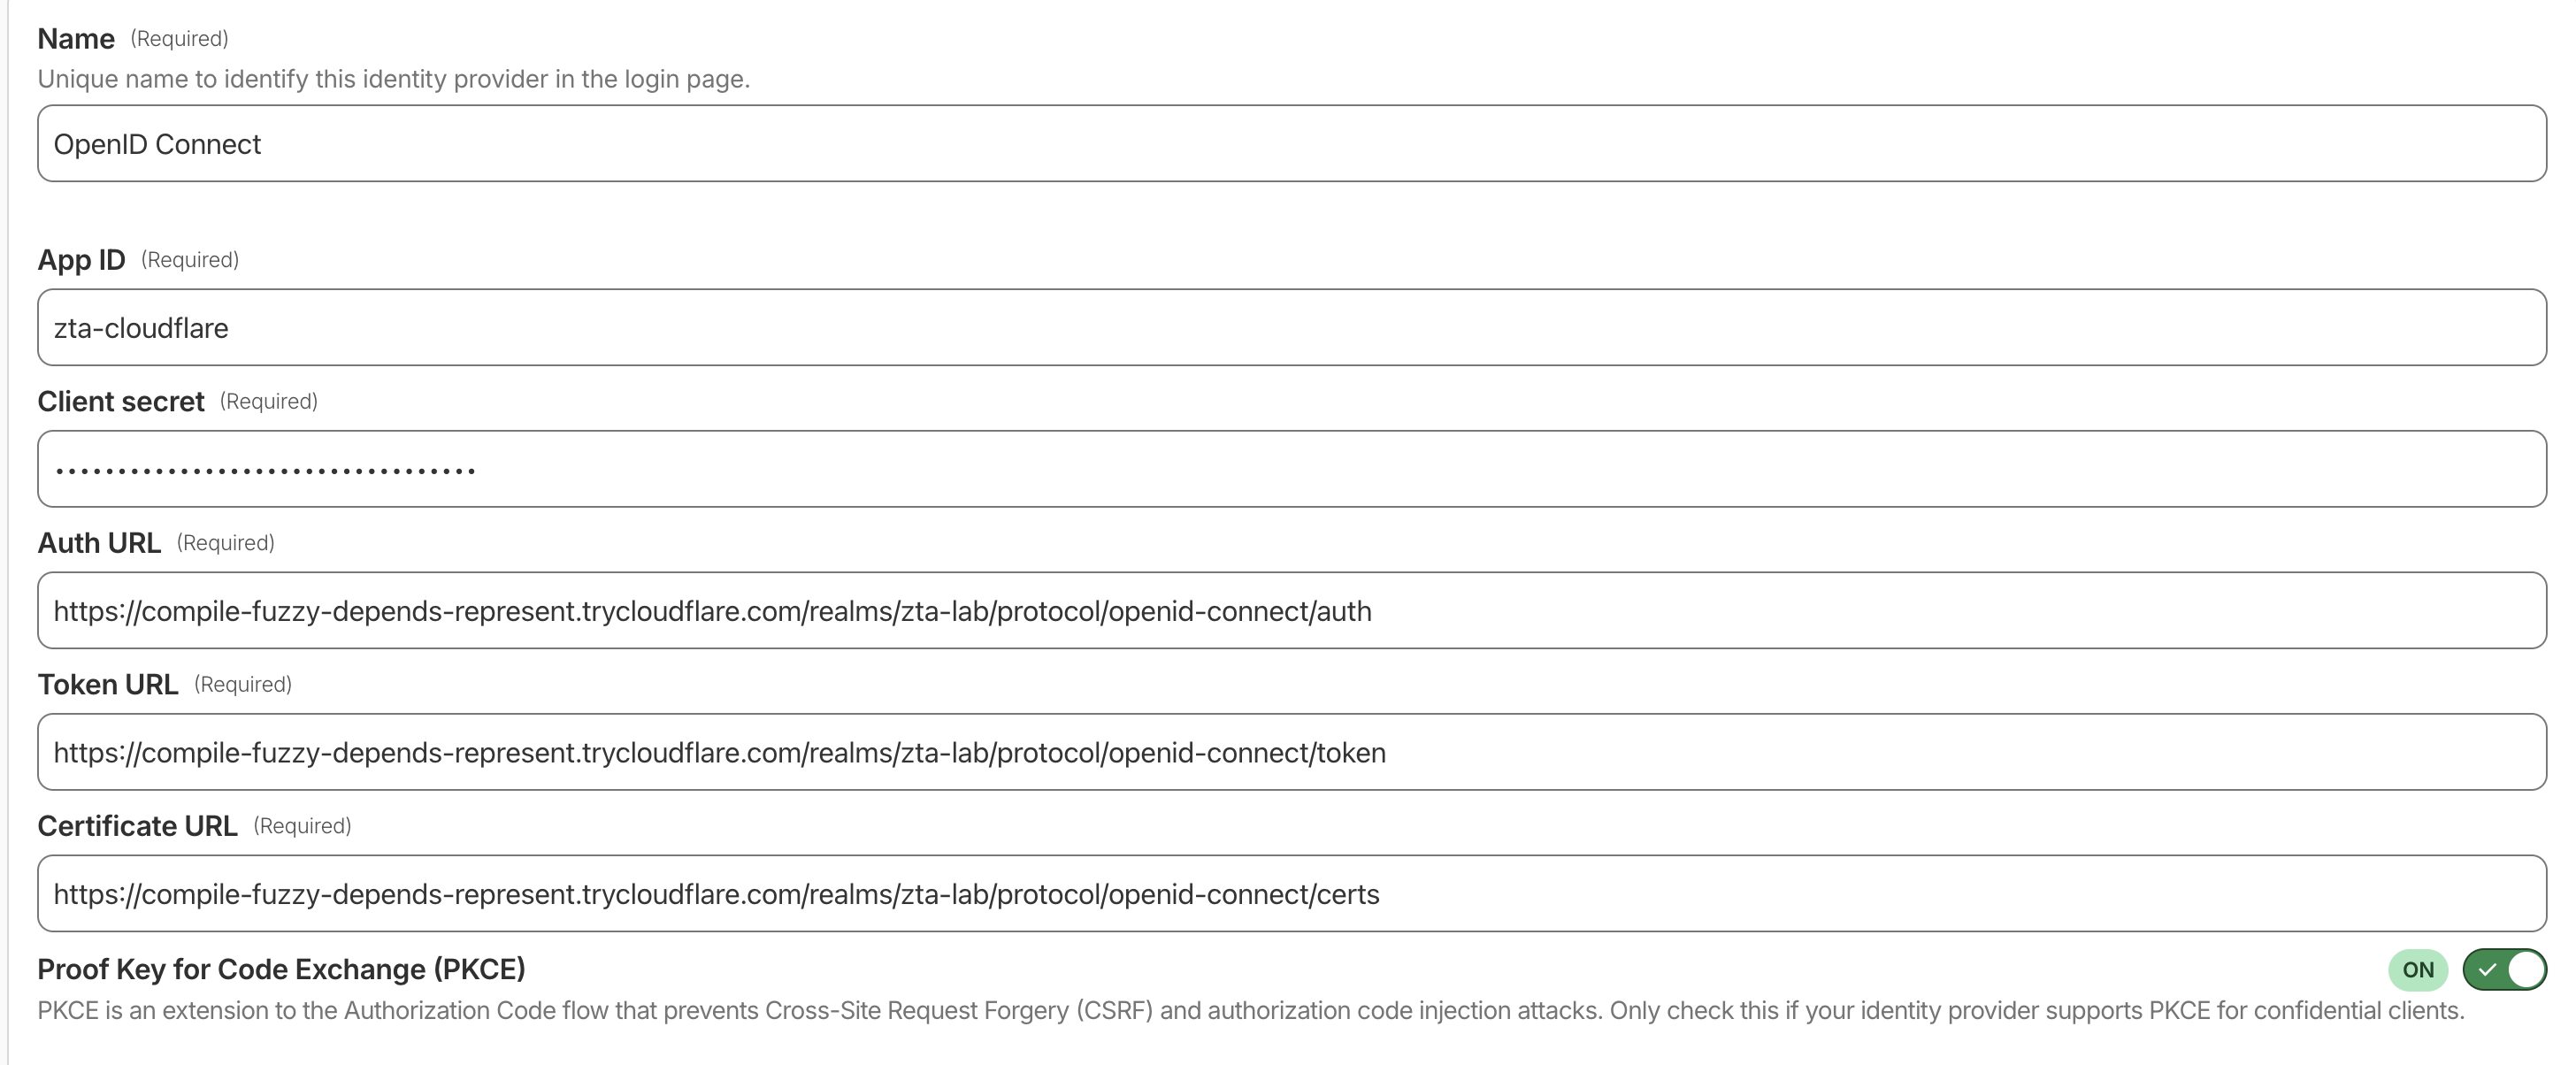
\includegraphics[width=0.5\textwidth]{contents/contents/image_6.png}
    \caption{Cấu hình IdP cho Cloudflare Zero Trust}
    \label{fig:example_image}
    
\end{figure}

\subsection{Xây dựng Access Policies cho các route bên trong app}
Sau khi hoàn tất liên kết định danh, hệ thống tiếp tục được ràng buộc bởi các chính sách truy cập theo nguyên tắc đặc quyền tối thiểu.
\begin{itemize}
    \item Tạo ứng dụng được bảo vệ trong Cloudflare Access, gắn với hostname hoặc đường dẫn cần kiểm soát.
    \item Khai báo chính sách \textbf{Allow} dựa trên danh tính người dùng, email, nhóm hoặc vai trò nhận được từ Keycloak.
    \item Bổ sung các điều kiện ngữ cảnh như quốc gia, địa chỉ IP hoặc yêu cầu xác thực lại khi cần để tăng mức độ bảo vệ.
    \item Thiết lập thứ tự ưu tiên giữa các chính sách \textbf{Allow}, \textbf{Deny} và \textbf{Bypass} để tránh xung đột trong quá trình đánh giá quyền truy cập.
    \item Một số policy được áp dụng: 
\end{itemize}

\begin{figure}[H]
    \centering
    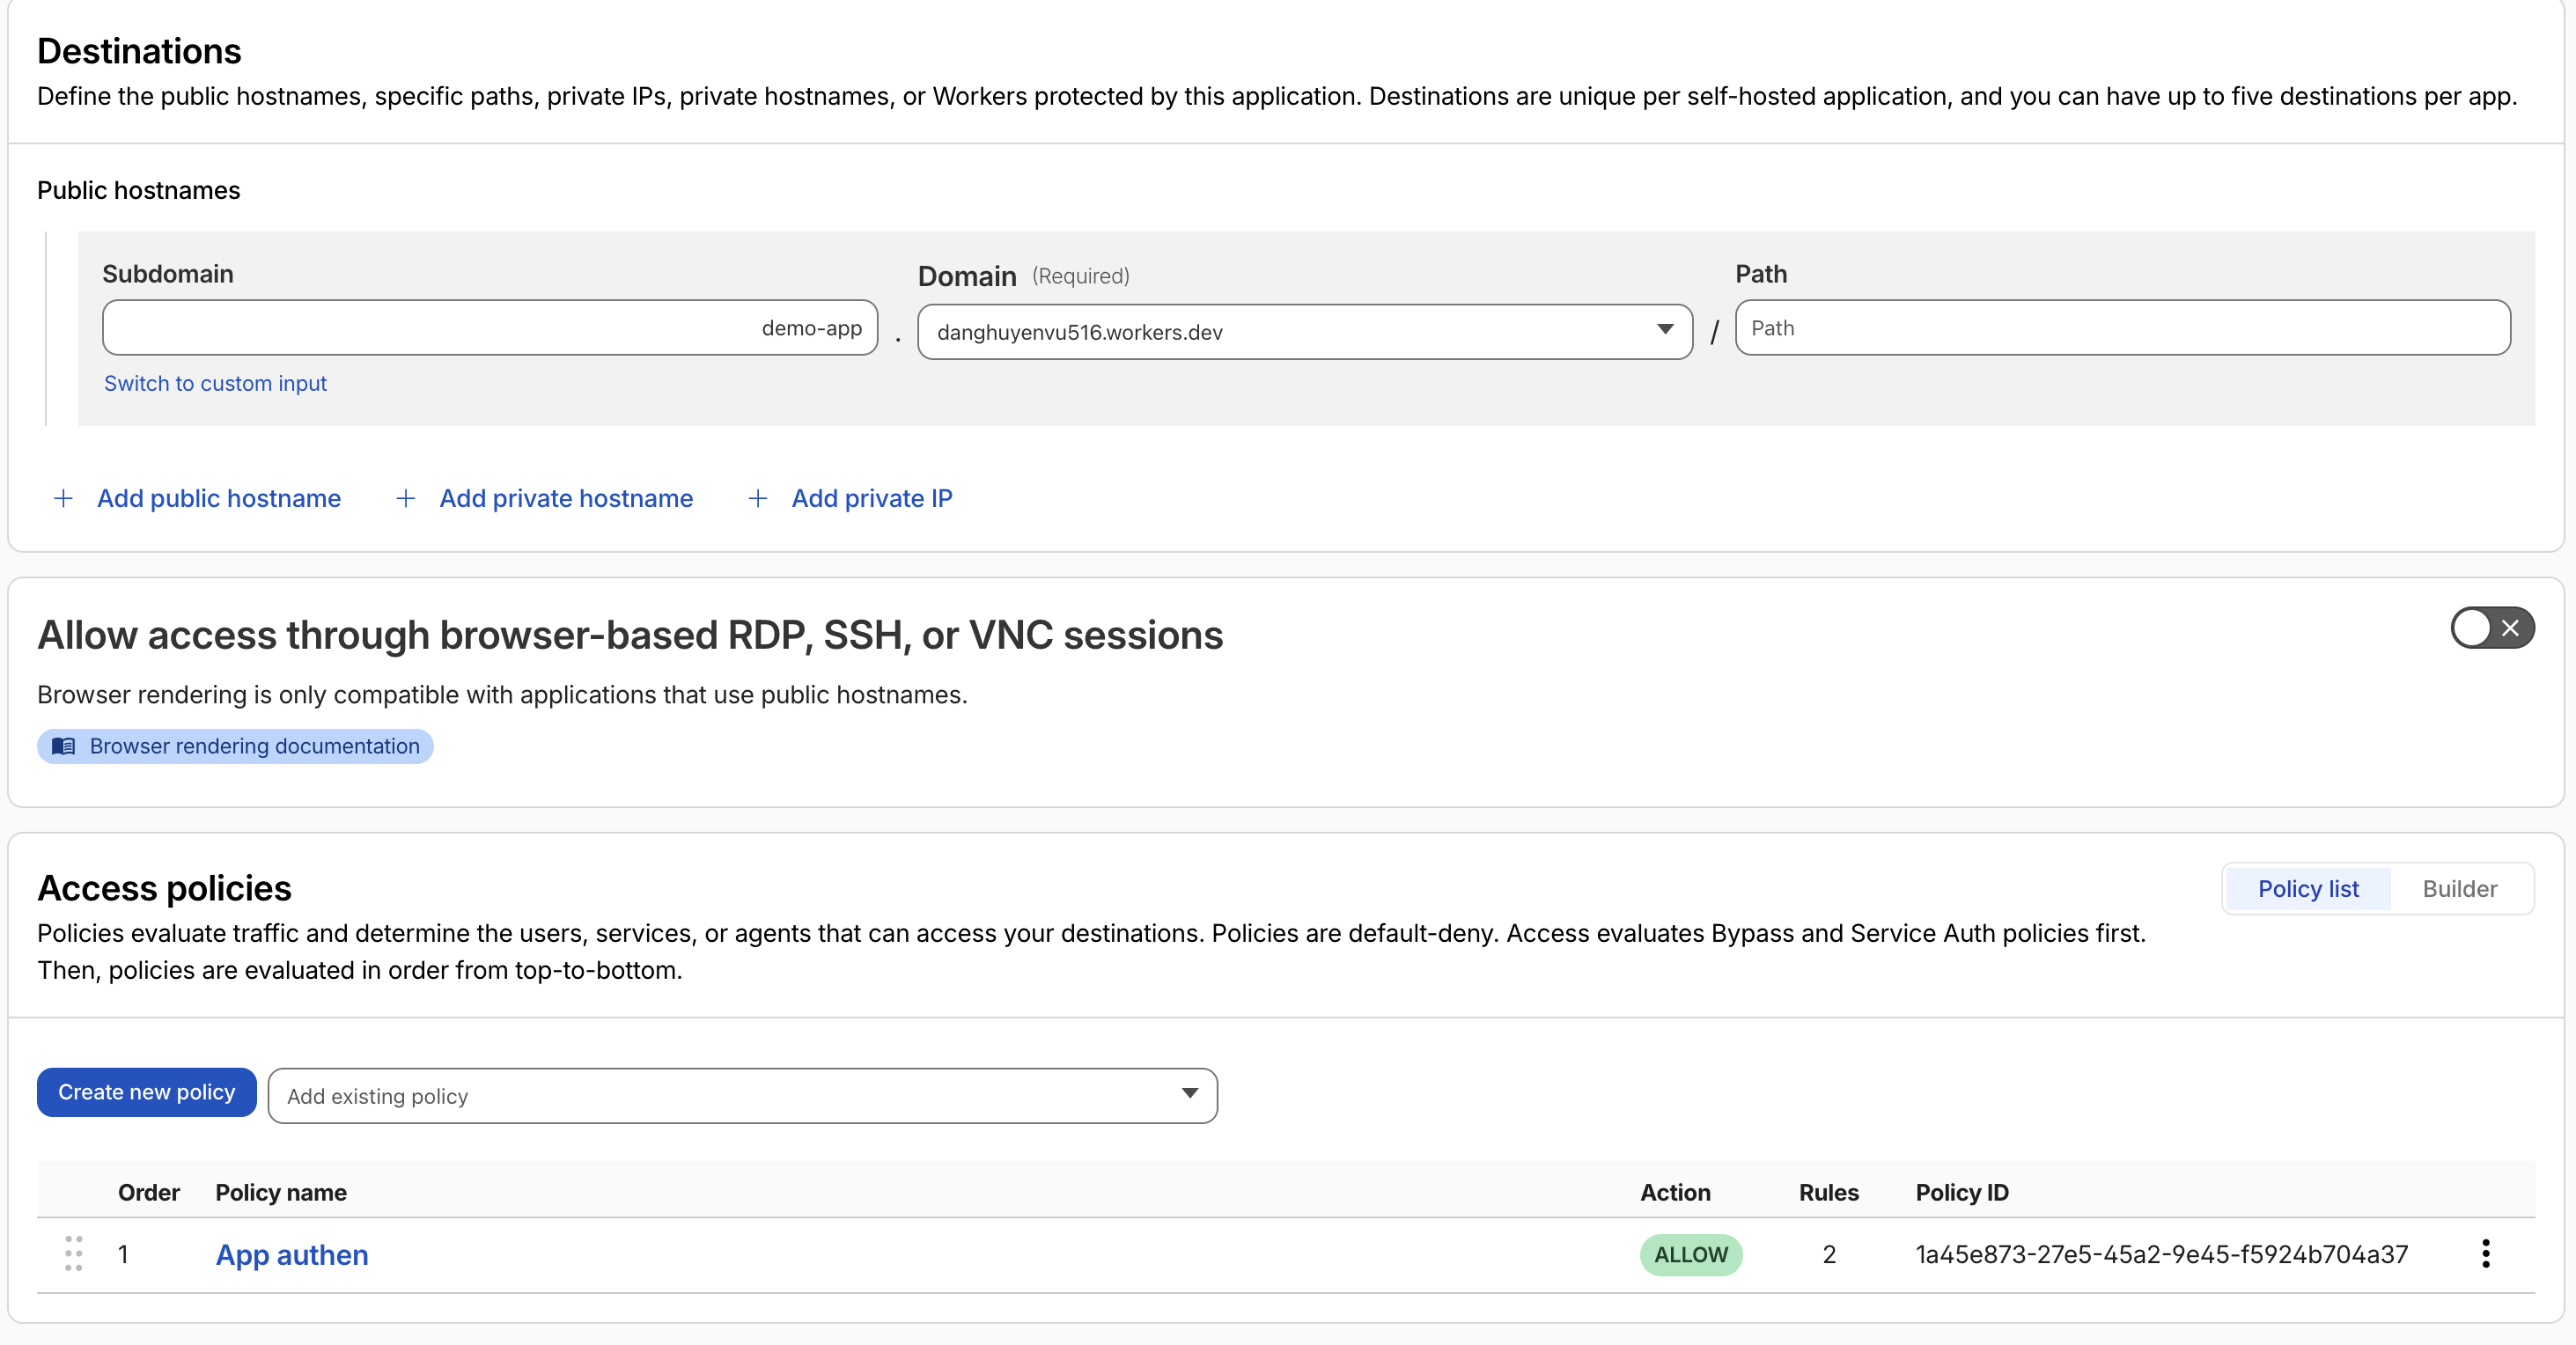
\includegraphics[width=0.5\textwidth]{contents/contents/image_12.png}
    \caption{Access policy cho Protected Application yêu cầu xác thực qua IdP}
    \label{fig:example_image}
    
\end{figure}

\begin{figure}[H]
    \centering
    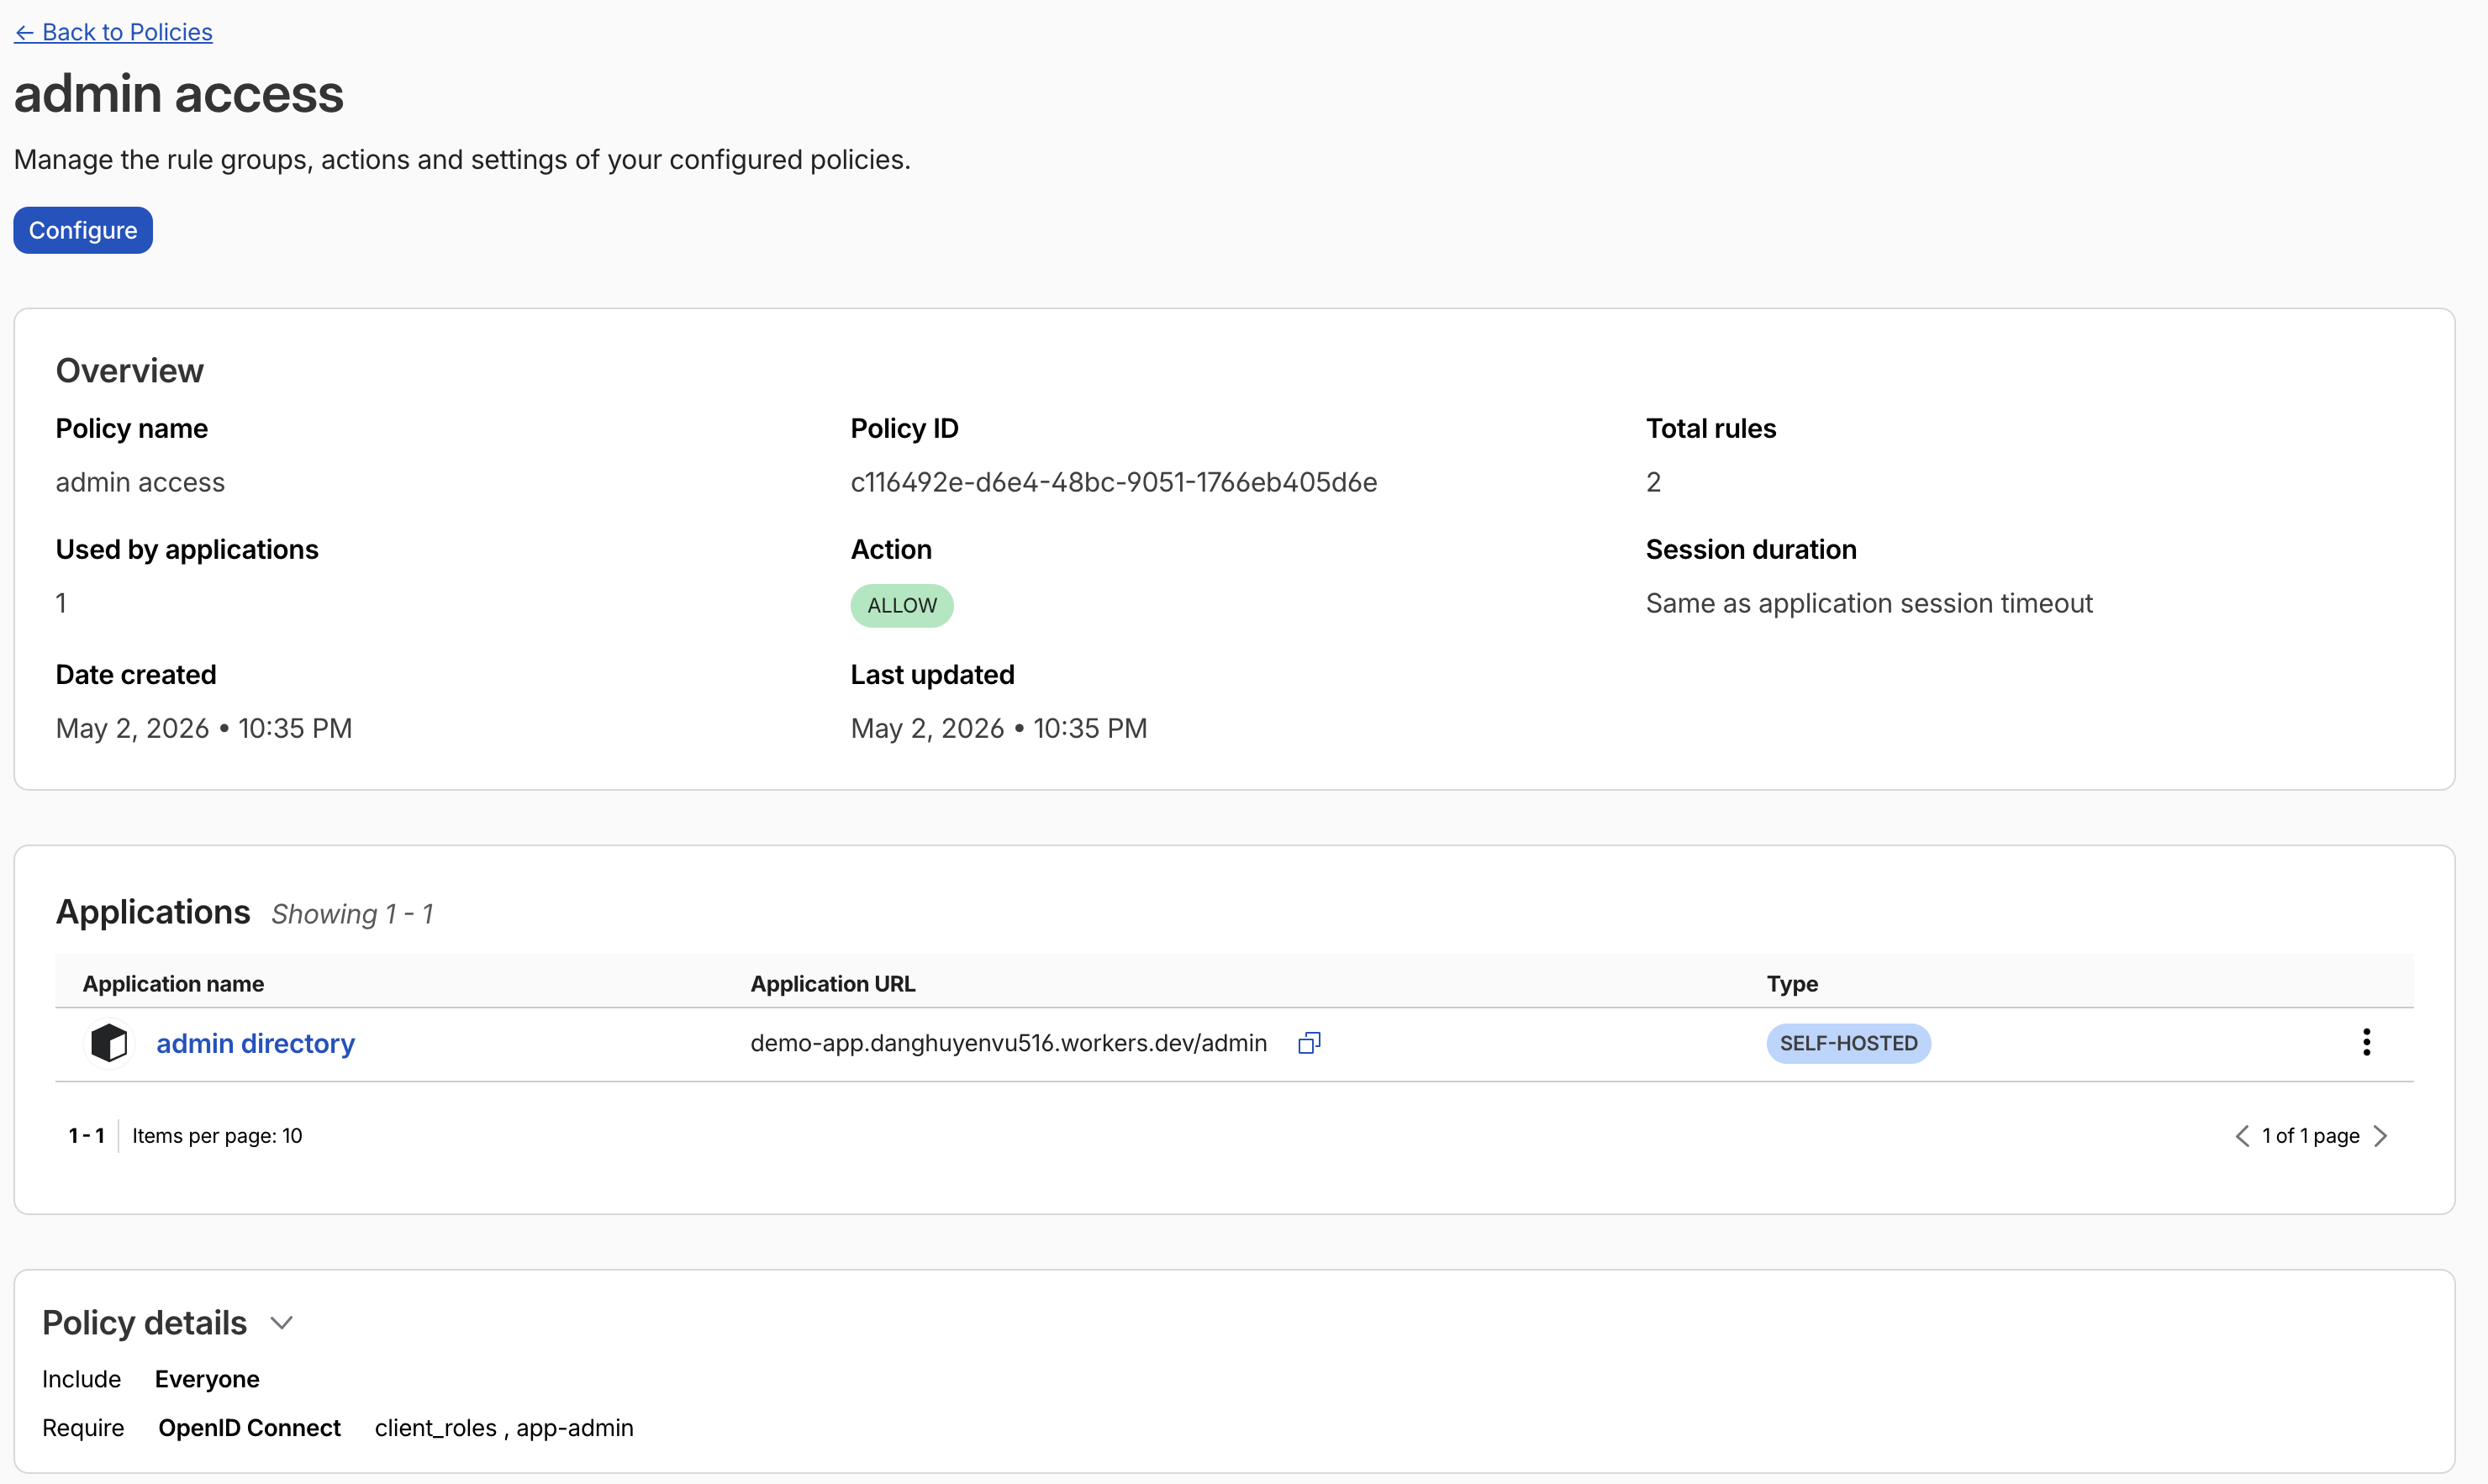
\includegraphics[width=0.5\textwidth]{contents/contents/image_19.png}
    \caption{Policy kiểm soát truy cập tài nguyên của admin}
    \label{fig:example_image}
    
\end{figure}

\begin{figure}[H]
    \centering
    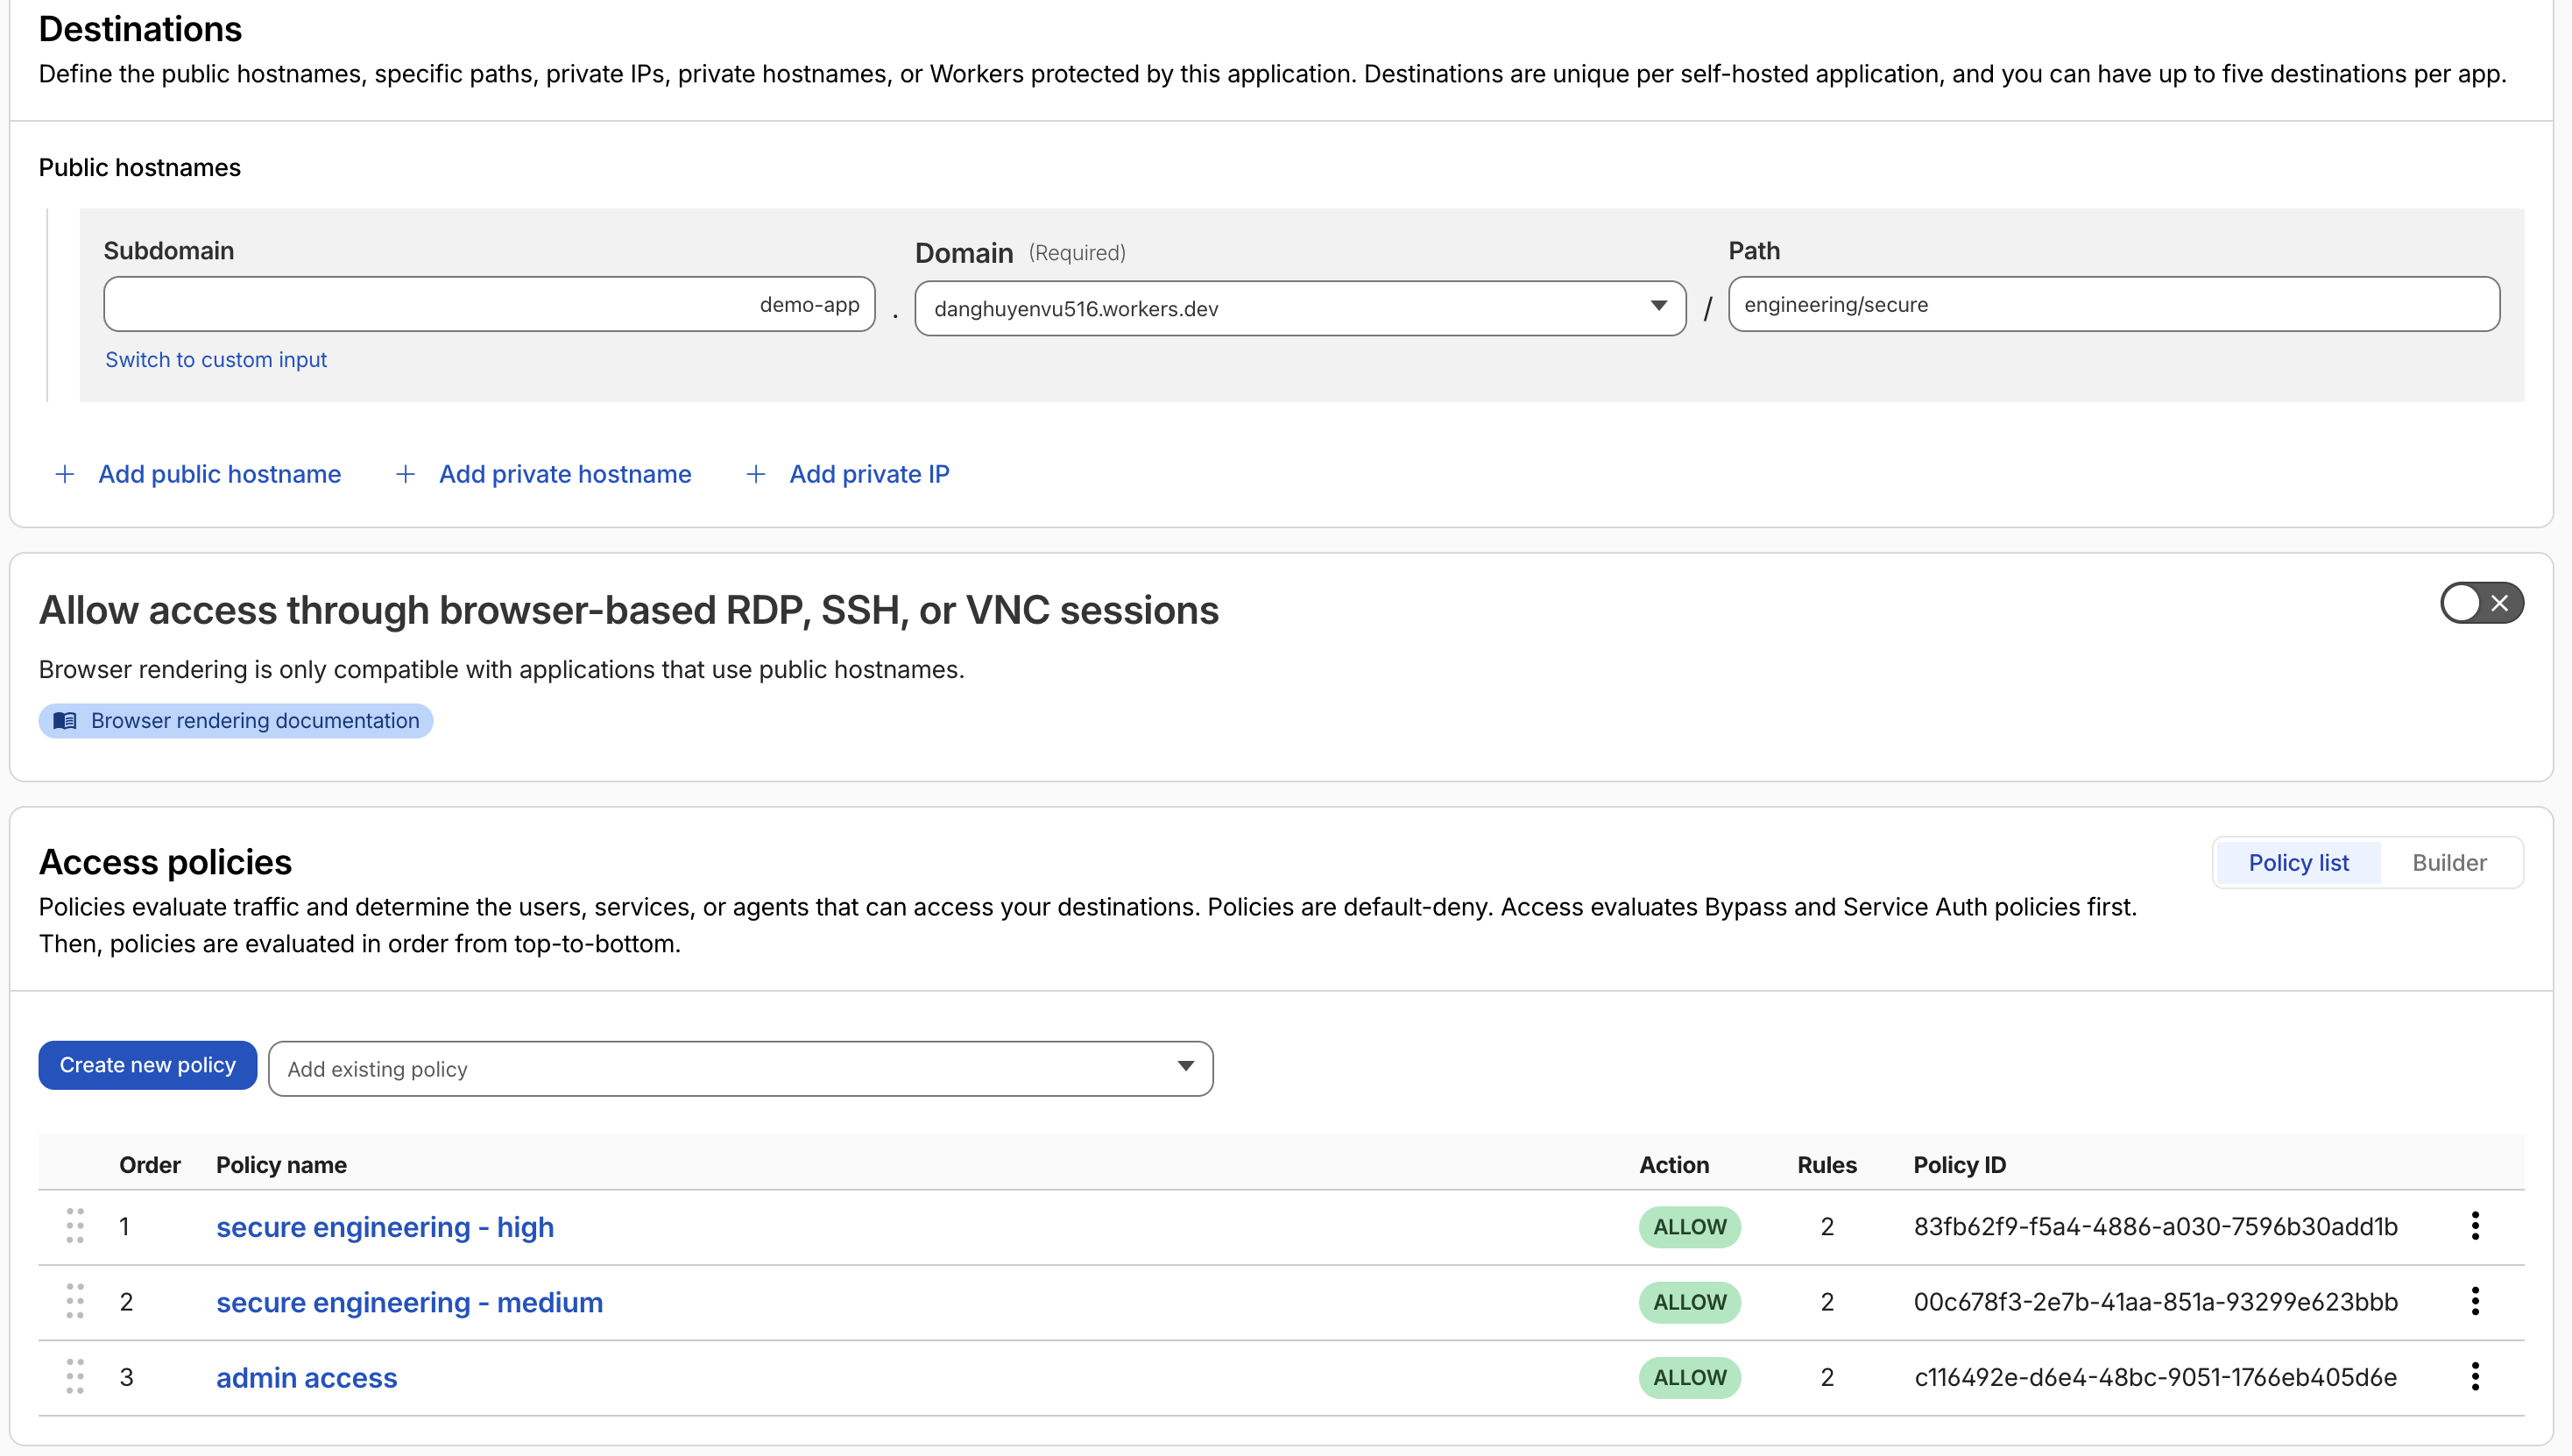
\includegraphics[width=0.5\textwidth]{contents/contents/image_20.png}
    \caption{Áp dụng policy cho /engineering/secure yêu cầu khắt khe hơn khi truy cập những tài nguyên quan trọng}
    \label{fig:example_image}
    
\end{figure}

\subsection{Kiểm thử luồng đăng nhập}
Luồng kiểm thử được thực hiện từ góc nhìn người dùng cuối nhằm xác nhận toàn bộ chuỗi xác thực và ủy quyền hoạt động đúng như thiết kế.
\begin{figure}[H]
    \centering
    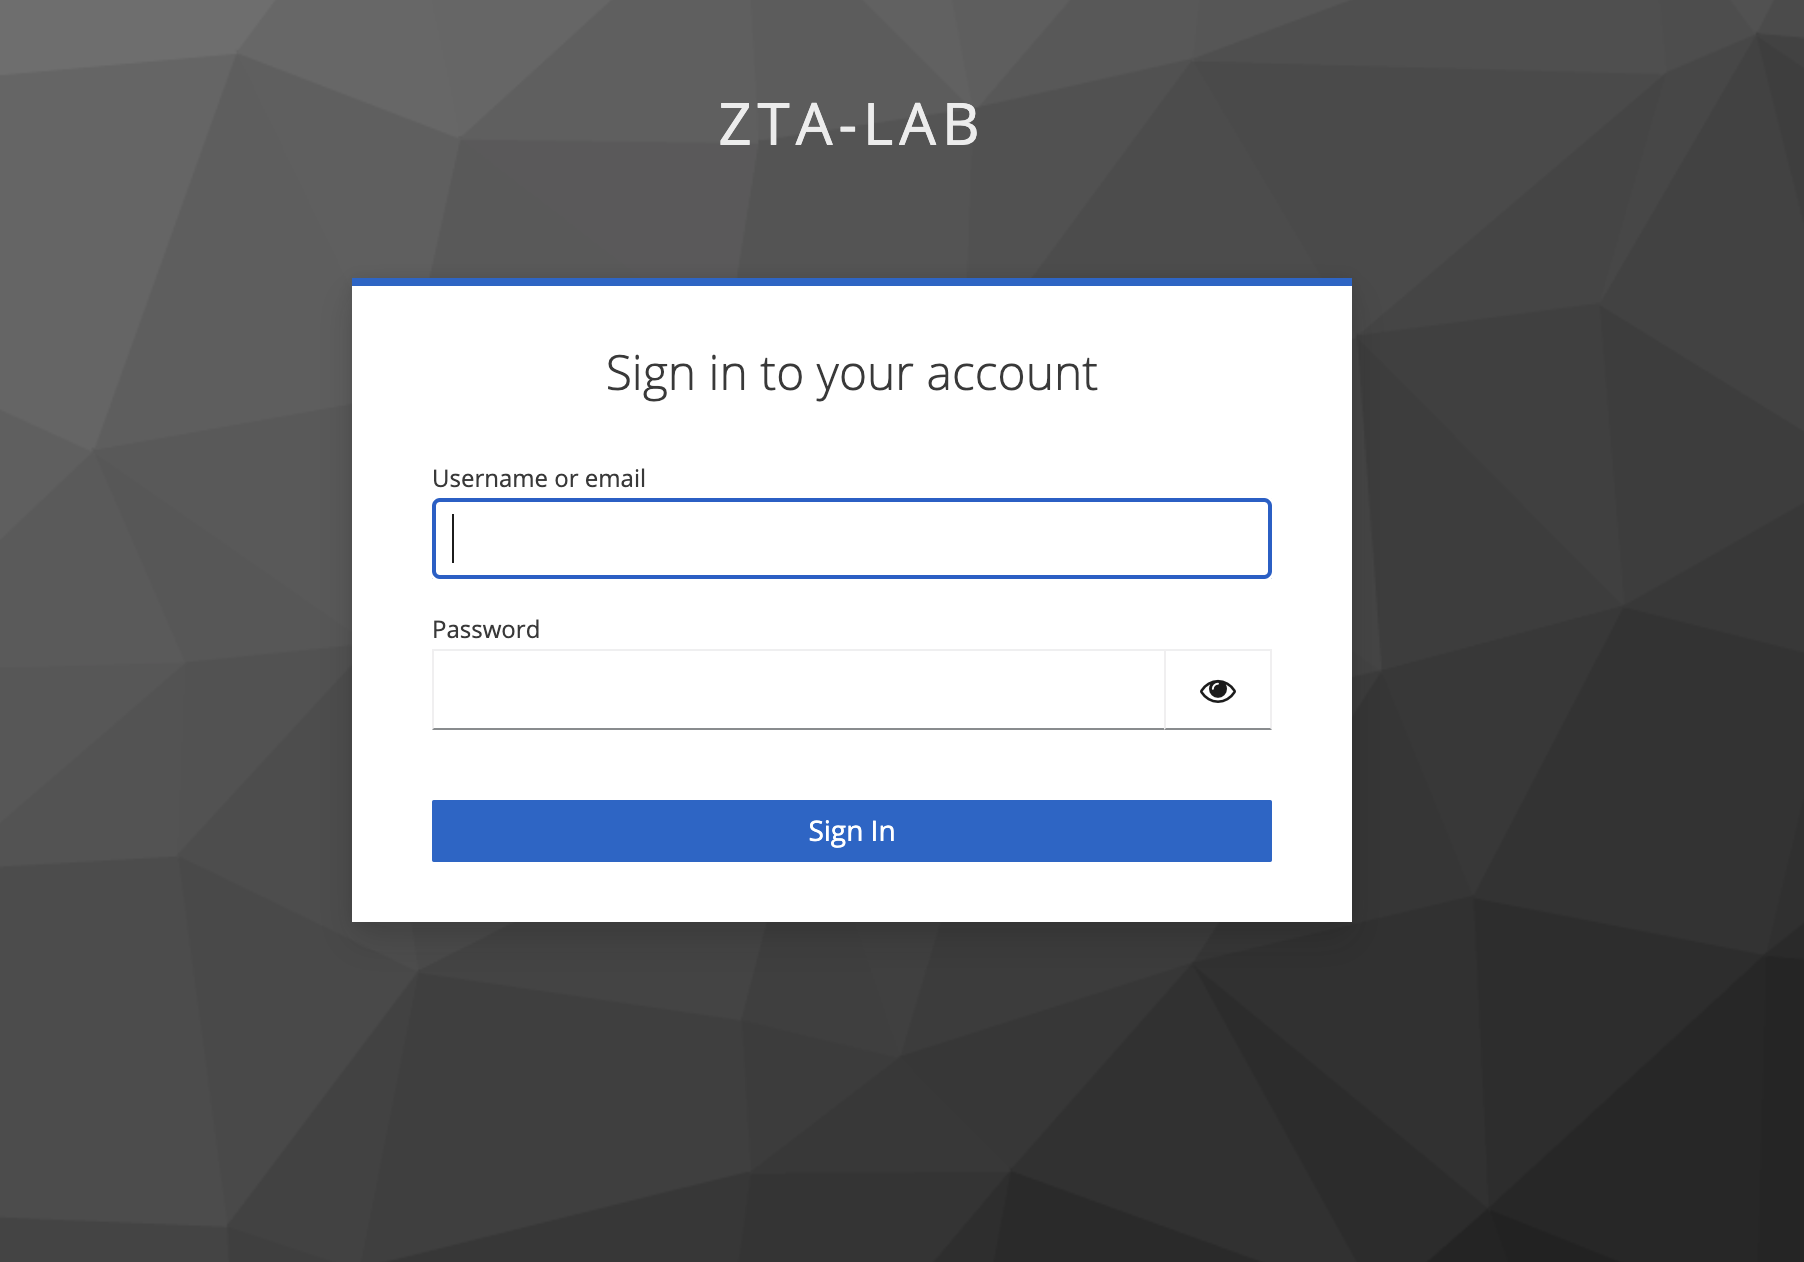
\includegraphics[width=0.5\textwidth]{contents/contents/image_13.png}
    \caption{Login page của Keycloak}
    \label{fig:example_image}
\end{figure}
Người dùng khi muốn truy cập ứng dụng web được bảo vệ nếu chưa được xác thực sẽ bị Cloudflare Access chặn lại tại lớp biên và điều hướng tới trang login của Keycloak để xác thực thông qua giao thức OIDC.

\begin{figure}[h]
    \centering
    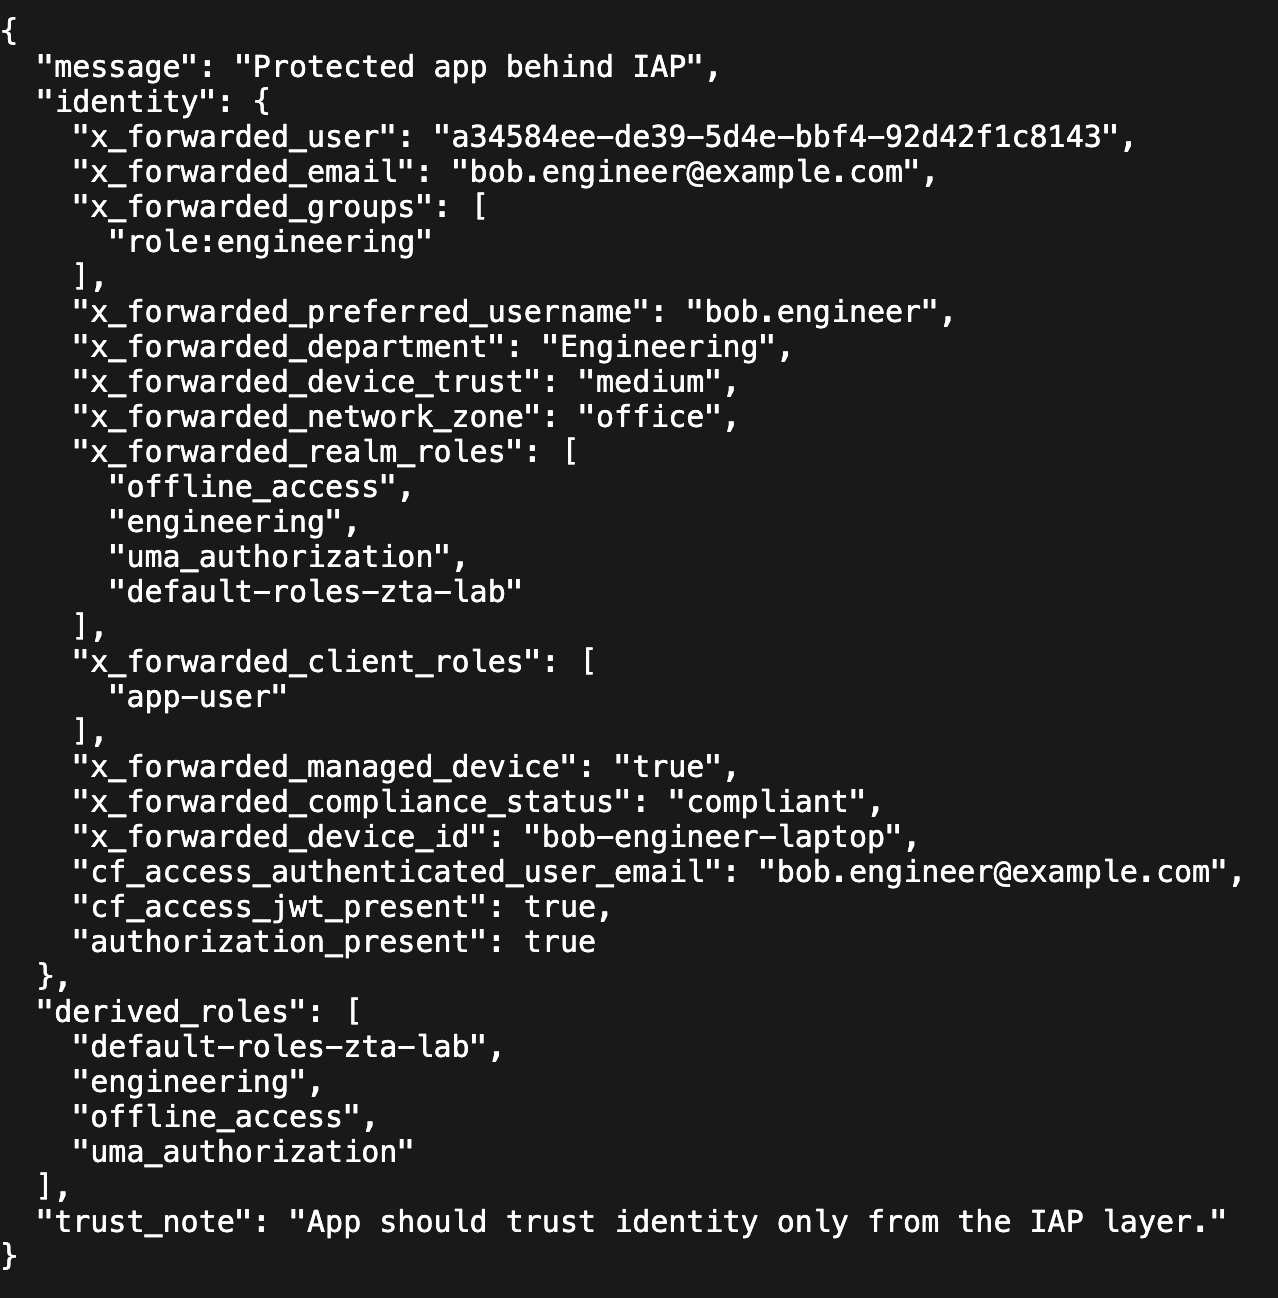
\includegraphics[width=0.5\textwidth]{contents/contents/image_14.png}
    \caption{Thông tin user khi đăng nhập thành công}
    \label{fig:example_image}
    
\end{figure}

Một người dùng muốn truy cập các tài nguyên không được phép sẽ bị chặn:
\begin{figure}[H]
    \centering
    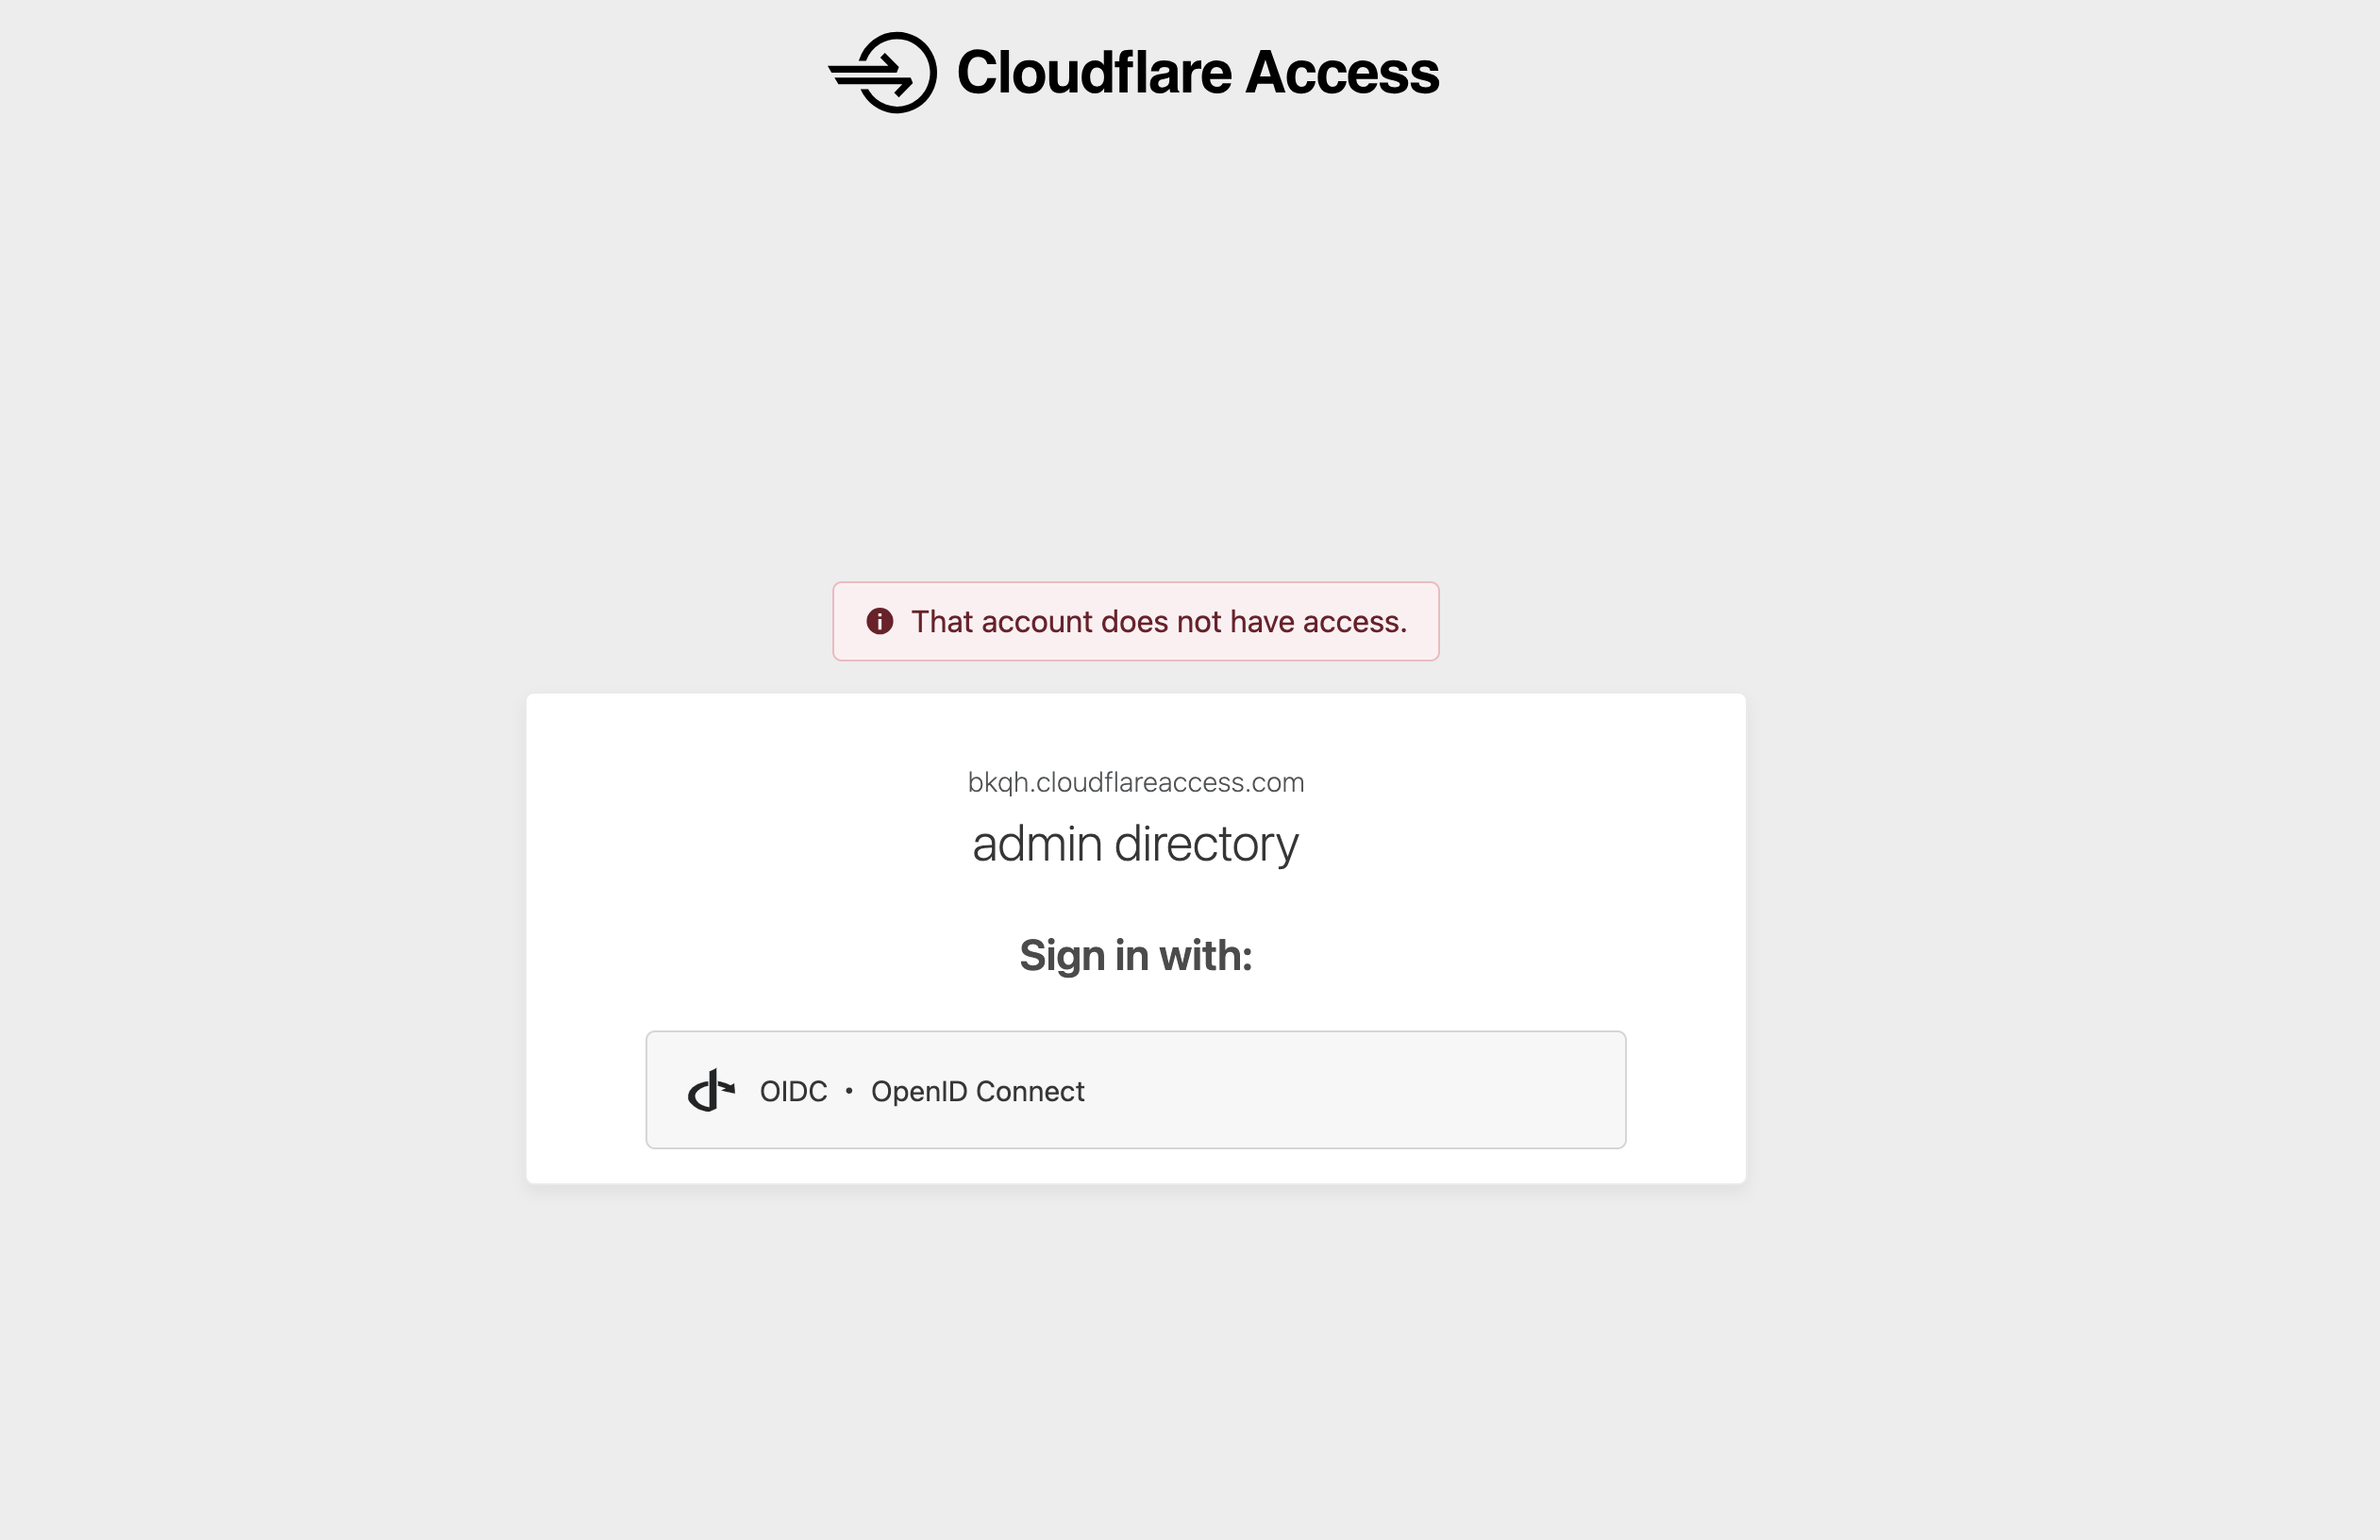
\includegraphics[width=0.5\textwidth]{contents/contents/image_18.png}
    \caption{Người dùng không đủ đặc quyền bị chặn khi truy cập directory yêu cầu đặc quyền cao với claim tương ứng}
    \label{fig:example_image}
    
\end{figure}

\begin{itemize}
    \item Người dùng truy cập ứng dụng được bảo vệ và bị Cloudflare Access chặn tại lớp biên.
    \item Cloudflare chuyển hướng người dùng sang trang đăng nhập Keycloak thông qua giao thức OIDC.
    \item Sau khi xác thực thành công, Keycloak trả mã hoặc token cho Cloudflare để hoàn tất phiên đăng nhập.
    \item Cloudflare đánh giá token cùng các Access Policies; nếu đạt điều kiện thì cấp quyền vào ứng dụng, ngược lại từ chối truy cập.
\end{itemize}

\subsection{Định hướng đánh giá}
Phần đánh giá tập trung vào cả tính đúng đắn của luồng xác thực lẫn hiệu quả bảo vệ tài nguyên.
\begin{itemize}
    \item \textbf{Đánh giá chức năng}: Kiểm tra khả năng đăng nhập thành công với người dùng hợp lệ và từ chối với người dùng không thuộc chính sách.
    \item \textbf{Đánh giá bảo mật}: Xem xét việc ẩn IP gốc nhờ Tunnel, khả năng chặn truy cập trực tiếp và hiệu quả của kiểm soát theo danh tính.
    \item \textbf{Đánh giá vận hành}: Ghi nhận độ thuận tiện khi cấu hình thử nghiệm bằng \texttt{trycloudflare}, đồng thời chỉ ra hạn chế của tunnel miễn phí trong triển khai dài hạn.
    \item \textbf{Đánh giá trải nghiệm}: Quan sát số bước đăng nhập, độ trễ chuyển hướng và tính minh bạch của luồng xác thực đối với người dùng cuối.
\end{itemize}


\section{KẾT LUẬN VÀ HƯỚNG PHÁT TRIỂN}

\subsection{Kết quả đạt được}
Dự án đã hoàn thành các mục tiêu đặt ra trong việc xây dựng hệ thống bảo mật theo mô hình Zero Trust, cụ thể:
\begin{itemize}
\item \textbf{Về kiến trúc}: Hiện thực hóa nguyên lý "Never Trust, Always Verify" thông qua lớp Identity-Aware Proxy (IAP). Chuyển đổi thành công sang mô hình \textbf{Serverless Edge}, loại bỏ rủi ro lộ IP máy chủ gốc.
\item \textbf{Về công nghệ}: Tích hợp hoàn chỉnh giao thức OIDC giữa Keycloak và Cloudflare. Triển khai thành công cơ chế \textbf{Identity Propagation}, chuyển hóa Claims từ IdP thành các Header định danh giúp ứng dụng biên nhận biết người dùng tức thời.
\item \textbf{Về bảo mật}: Thiết lập thành công cơ chế phân quyền động (Dynamic Authorization) tại tầng biên, đảm bảo tài nguyên chỉ được thực thi sau khi vượt qua các kiểm tra nghiêm ngặt về danh tính và ngữ cảnh.
\end{itemize}

\subsection{Hạn chế của hệ thống}
Mặc dù đạt được các mục tiêu chính, hệ thống vẫn tồn tại một số hạn chế:
\begin{itemize}
\item \textbf{Phụ thuộc hạ tầng trung gian}: Hệ thống phụ thuộc lớn vào tính sẵn sàng của Cloudflare. Nếu có sự cố tại các Node của Cloudflare, việc truy cập ứng dụng có thể bị gián đoạn.
\item \textbf{Giới hạn của môi trường Runtime}: Cloudflare Workers có giới hạn về dung lượng bộ nhớ và thời gian thực thi (CPU time), gây khó khăn nếu ứng dụng cần xử lý các tác vụ tính toán nặng.
\end{itemize}

\subsection{Ưu điểm và Nhược điểm}
\begin{table}[H]
\centering
\caption{Đánh giá ưu và nhược điểm của giải pháp}
\begin{tabular}{|p{7cm}|p{7cm}|}
\hline
\textbf{Ưu điểm} & \textbf{Nhược điểm} \\ \hline
Tối ưu hiệu năng nhờ xử lý tại Edge (QUIC, HTTP/3). & Đòi hỏi kiến thức chuyên sâu về Serverless và quản trị IdP. \\ \hline
Bề mặt tấn công cực nhỏ (Zero Attack Surface) do không có IP công khai. & Khó khăn trong việc Debug và theo dõi Logs chi tiết hơn so với Server truyền thống. \\ \hline
Chi phí vận hành thấp, khả năng tự động mở rộng (Auto-scaling) linh hoạt. & Phụ thuộc vào chính sách giá và giới hạn của nhà cung cấp Cloud. \\ \hline
\end{tabular}
\end{table}
\newpage
\subsection{Hướng phát triển tương lai}
Để hoàn thiện hệ thống, các hướng nghiên cứu tiếp theo bao gồm:
\begin{itemize}
\item \textbf{Tăng cường Context-aware}: Tích hợp thêm các tín hiệu về trạng thái thiết bị (Device Posture) và hành vi người dùng để đưa ra quyết định truy cập chính xác hơn.
\item \textbf{Mở rộng lưu trữ tại biên}: Sử dụng Cloudflare D1 (SQL) hoặc Workers KV để xây dựng các ứng dụng Full-stack hoàn chỉnh chạy hoàn toàn trên mô hình Zero Trust Edge.
\item \textbf{Tự động hóa chính sách}: Nghiên cứu áp dụng Infrastructure as Code (Terraform) để quản lý đồng bộ các Access Policies và Keycloak Clients.
\end{itemize}

\newpage
\begin{thebibliography}{99}

\bibitem{nist} 
S. Rose, O. Borchert, S. Mitchell, and S. Connelly, ``Zero Trust Architecture,'' \textit{NIST Special Publication 800-207}, Aug. 2020. [Online]. Available: https://doi.org/10.6028/NIST.SP.800-207

\bibitem{oidc} 
N. Sakimura et al., ``OpenID Connect Core 1.0 incorporating errata set 1,'' \textit{The OpenID Foundation}, Nov. 2014.

\bibitem{cloudflare_zta} 
Cloudflare, ``What is a Zero Trust Architecture?'' \textit{Cloudflare Learning Center}. [Online]. Available: https://www.cloudflare.com/learning/security/glossary/what-is-zero-trust/

\bibitem{keycloak_auth} 
Red Hat, ``Keycloak Server Administration Guide,'' \textit{Keycloak.org}. [Online]. Available: https://www.keycloak.org/docs/latest/server\_admin/

\bibitem{workers_docs} 
Cloudflare, ``Cloudflare Workers documentation,'' \textit{Cloudflare Developers}. [Online]. Available: https://developers.cloudflare.com/workers/

\end{thebibliography}
\newpage
\section*{PHỤ LỤC: TÀI LIỆU VÀ MÔI TRƯỜNG PHÁT TRIỂN}

\subsection*{1. Tài liệu tham khảo}

\begin{itemize}
\item \textbf{NIST Special Publication 800-207}: Tài liệu tiêu chuẩn quốc gia định nghĩa kiến trúc Zero Trust (ZTA) và các thành phần cốt lõi.
\item \textbf{Cloudflare Zero Trust Documentation}: Hướng dẫn kỹ thuật triển khai Identity-Aware Proxy (IAP), cấu hình OIDC Identity Provider và Access Policies.
\item \textbf{Keycloak Server Administration Guide}: Tài liệu quản trị Keycloak, bao gồm cấu hình Client OIDC và Protocol Mappers để tùy chỉnh claims trong token.
\item \textbf{OpenID Connect Core 1.0}: Đặc tả chính thức của giao thức OIDC.
\item \textbf{RFC 7519 -- JSON Web Token (JWT)}: Tiêu chuẩn kỹ thuật về cấu trúc và cơ chế bảo mật của JSON Web Token.
\end{itemize}

\subsection*{2. Môi trường phát triển}

\begin{itemize}
\item \textbf{Nền tảng thực thi}: Cloudflare Workers (Serverless) trên môi trường V8 JavaScript.
\item \textbf{Hệ điều hành}: Windows 11 / macOS (môi trường phát triển); Docker cho việc triển khai Keycloak trong giai đoạn thử nghiệm.
\item \textbf{Công cụ phát triển}:
  \begin{itemize}
  \item Visual Studio Code với các extension hỗ trợ JavaScript/TypeScript và Cloudflare Workers.
  \item \texttt{Wrangler CLI} (công cụ chính thức của Cloudflare) dùng để phát triển, preview và triển khai.
  \end{itemize}
\item \textbf{Công cụ kiểm thử}: Postman (kiểm tra luồng xác thực, redirect và cấu trúc header/token).
\end{itemize}

\subsection*{3. Thư viện và công nghệ mã nguồn mở}

\begin{itemize}
\item \textbf{Keycloak}: Giải pháp IAM mã nguồn mở, hỗ trợ đầy đủ OIDC, OAuth 2.0 và SAML.
\item \textbf{Cloudflare Wrangler}: Bộ công cụ phát triển và triển khai Cloudflare Workers.
\item \textbf{Web APIs tiêu chuẩn} (được hỗ trợ natively trong Cloudflare Workers):
  \begin{itemize}
  \item \texttt{Fetch API} -- Xử lý HTTP requests.
  \item \texttt{Headers Interface} -- Trích xuất thông tin từ \texttt{Cf-Access-Jwt-Assertion}.
  \item \texttt{Web Crypto API} -- Kiểm tra chữ ký và xử lý token (nếu cần).
  \end{itemize}
\end{itemize}

\subsection*{4. Mã nguồn tham khảo}

\begin{itemize}
\item Cloudflare Access Headers samples (xử lý JWT từ header \texttt{Cf-Access-Jwt-Assertion}).
\item Keycloak Custom Protocol Mapper examples (thêm Group/Role vào ID Token).
\item Các ví dụ triển khai Zero Trust với OIDC trên Cloudflare Workers từ tài liệu chính thức và cộng đồng.
\end{itemize}



\end{document}